\documentclass[12pt,a4paper,oneside, titlepage]{article}
\usepackage[left=2cm,right=2cm,top=2cm,bottom=2cm]{geometry}
\usepackage[pdftex]{graphicx}
\usepackage[final]{pdfpages}
\usepackage[frenchb]{babel}
\usepackage{xspace}
\usepackage{lmodern}
\usepackage[T1]{fontenc}
\usepackage[utf8]{inputenc}
\usepackage{cite}
\usepackage{hyperref}
\usepackage{amsmath}
\usepackage{amssymb}
\usepackage{amsthm}
\usepackage{booktabs}% http://ctan.org/pkg/booktabs
\usepackage{textcomp}% symbole degré
\newcommand{\tabitem}{~~\llap{\textbullet}~~}
\begin{document}
\newcommand{\spherotitle}[2]{
\begin{titlepage}
\begin{center}

\includegraphics[scale=1.50]{../UMONS.jpg}\\[0.4cm]

\includegraphics[scale=0.30]{../FS_Logo.jpg}\\[3cm]
{\Large Un réseau de neurones pour la}\\

\includegraphics[scale=0.30]{../sphero.jpg}\\
\rule{8cm}{0.5mm}\\[0.5cm]
{\huge \bfseries #1}\\[0.2cm]
\rule{8cm}{0.5mm}\\[7cm]
% Author and supervisor. Come from http://www.jujens.eu/posts/2013/Oct/20/latex-page-garde/
    \begin{minipage}{0.4\textwidth}
      \begin{flushleft} \large
        Jason \textsc{Bury}\\
        130538\\
        Master 1 en\\Science-informatique\\
      \end{flushleft}
    \end{minipage}
    \begin{minipage}{0.4\textwidth}
      \begin{flushright} \large
        \emph{Codirecteurs :}~~\\M. Pierre \textsc{Hauweele}\\M. Hadrien \textsc{Mélot}\\
        \emph{Rapporteur : }~~\\M. Tom \textsc{Mens}
      \end{flushright}
    \end{minipage}
   \vfill
  {\large #2}
\end{center}
\end{titlepage}
}
\newcommand{\terminologie}{
\begin{figure}
 \begin{center}
 \underline{\hypertarget{terminologie}{Terminologie}}\\
 \begin{tabular}{|l|l|}
  \hline
  Terme & Nom anglais complet\\
  \hline
  ANN & Artificial Neural Network\\
  ELM & Extreme Learning Machine\\
  FNN & Feedforward Neural Networks\\
  MLP & Multilayer Perceptron\\
  RBF & Radial Basis Function\\
  CNN & Convolutional neural Network\\
  RNN & Recurrent Neural Network\\
  SRN & Simple Recurrent Network\\
  ESN & Echo State Network\\
  LSM & Liquid State Machine\\
  SNN & Spiking Neural Network\\
  LSTM & Long Short-Term Memory\\
  BRNN & Bi-directional Recurrent Neural Network\\
  RMLP & Recurrent Multilayer Perceptron\\
  \hline
 \end{tabular}
 \end{center}
 \caption{Terminologie des réseaux de neurones}
 \label{terminologie}
\end{figure}
}

\newcommand{\termi}[1]{\hyperlink{terminologie}{\uppercase{#1}} }
\newcommand{\rbf}{\termi{rbf}}
\newcommand{\mlp}{\termi{mlp}}
\newcommand{\rmlp}{\termi{rmlp}}
\newcommand{\srn}{\termi{srn}}
\newcommand{\ann}{\termi{ann}}
\newcommand{\lsm}{\termi{lsm}}

\newcommand{\rna}{\hyperlink{rna}{RNA} }
\newcommand{\ubf}[1]{\textbf{\underline{#1}}}
\newcommand{\enum}[1]{\og #1 \fg}%{\og\textbf{#1}\fg}
\newcommand{\captionsource}[2]{
  \caption[{#1}]{
    #1
    \\\hspace{\linewidth}
    \textbf{Source:} #2
  }
}

\newcommand{\partiel}[2]{\frac{\partial #1}{\partial #2}}
\newtheorem{definition}{Définition}
\newtheorem{thm}{Théorème}
\spherotitle{Rapport}{Année 2016-2017}
\tableofcontents
\newpage
\section{Introduction}
\subsection{Énoncé}
Ce projet consiste à implémenter un \emph{réseau de neurones artificiels} \hypertarget{rna}{(RNA)} pour commander la Sphero.
Il devra effectuer n'importe quelle trajectoire qui peut être à grande vitesse et aussi gérer les dérapages.
La Sphero sera commandée sur un sol plat sans obstacle.
\subsection{Présentation de la Sphero}
La Sphero est une boule robotisée téléguidée, connectée par Bluetooth.
À l'intérieur, il y a deux moteurs: un pour faire tourner le poid et l'autre pour changer l'orientation de l'appareil.
En faisant tourner le poid, la Sphero déplace son centre de gravité en dehors de sa base de sustentation, faisant ainsi rouler l'appareil.
\subsection{Avantages d'un réseau de neurones}
\begin{itemize}
 \item \textbf{parallélisme}: L'apprentissage et la génération de vecteur de sortie est massivement parallélisable dans un RNA.\cite{corelet,Haykin}
 \item \textbf{Généralisation}: Répond de manière raisonnable à une entrée non rencontrée durant la phase d'apprentissage.\cite{statistica,Haykin}
 \item \textbf{Approximation non-linéaire}: Les RNA présentés dans ce rapport sont des approximateurs universels de fonctions non-linéaires.\cite{Haykin}
 \item \textbf{Adaptabilité}: Un RNA avec apprentissage on-line s'adapte aux changements dans le système.\cite{Haykin}
 \item \textbf{Boite noire}: Un RNA agit comme une boite noire. L'utilisateur n'a pas besoin de connaitre le fonctionnement du réseaux.
 \item \textbf{Tolérance au bruit}: Le bruitage dans la phase d'apprentissage impacte peu les performances d'un RNA.\cite{Haykin}
\end{itemize}
C'est grâce à ces avantages qu'un réseaux de neurones artificiels peut être intéressant pour commander la Sphero.
En effet, Il est très difficile de générer les commandes de manières analytique fidèle à la réalité à cause des trop nombreux paramètres à gèrer (Centre de gravité changeant, frottement, dérapages, équilibre, défauts,...).
Grâce au fait qu'un RNA agit comme une boite noire et est approximateur universel de fonction, nous pouvons nous passer de la conception d'un simulateur ou d'une tentative de formule analytique pour génerer les commandes.
De plus, si l'apprentissage se fait on-line, le réseau de neurones pourra s'adapter si le coefficient de frottement du sol change ou si il y une modification à la Sphero.
Et enfin, nous aurons invévitablement des bruitages dans les données fournies par les capteurs.

\newpage
\section{Théorie}
\subsection{Modèles de réseaux de neurones artificiels}
\terminologie
Tout d'abord, analysons les différents modèles de réseau de neurones artificiels éxistants afin de pouvoir sélectionner celui qui convient le mieux à notre application.
Les plus connus d'entre eux sont le perceptron multi-couche et la fonction à base radiale, tous deux non récurrents.
Ensuite nous verrons les réseaux de neurones récurrents qui approximent des fonctions qui peuvent dépendre de toutes les entrées précédentes.
Les terminologies utilisées proviennent de la littérature anglophone et tous ceux rencontrés sont répertoriés à la table \ref{terminologie}.
\newcommand{\ssstitle}[1]{\begin{center}\large\underline{#1}\normalsize\end{center}}
\subsection{Perceptron mutli-couches (MLP)}
\subsubsection{Neurone}
La Figure \ref{neuronemlp} schématise le travail d'un neurone d'indice $k$.
\begin{figure}
 \centering
 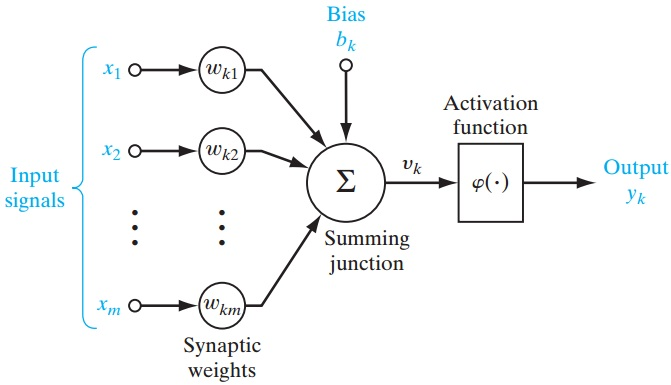
\includegraphics[scale=0.5]{../figures/neurone.jpg}
 \caption{Un neurone artificiel. \textbf{Source}: Haykin\cite{Haykin}}
 \label{neuronemlp}
\end{figure}
Un neurone effectue tout d'abord une somme pondérée de ses entrées \[v_k = b_k+\sum_{j=1}^{m}x_{j}w_{kj}\] où $x$ est le vecteur d'entrée de dimensions $m$.\\
Chaque terme $x_j$ est mutiplié par un poids $w_{kj}$.
Ce sont les poids qui seront modifiés lors de la phase d'apprentissage.
Le biais $b_k$ est souvent ajouté à la pondération.
Mais pour simplifier les formules, nous pouvons considèrer $b_k$ comme étant l'entrée $x_0 = 1$ de poid fixe $w_{k0} = 1$.
Et la somme pondérée est donc maintenant de la forme \[v_k = \sum_{j=0}^{m}x_{j}w_{kj}\]
Ensuite le neurone applique la \emph{fonction d'activation} $\phi$ sur la somme pondérée.
Le domaine de $y$ est généralement $[0,1]$ ou $[-1,1]$.\cite{Haykin,statistica}
La fonction $\phi$ utilisée dépend du problème qu'on veut résoudre (Figure \ref{mlpfonc}).
\begin{figure}
 \centering
 %insert tableau de statistica here
 \textbf{Fonctions d'activations.} (fonction de $x$)\\
 \begin{tabular}{|l|c|c|}
  Nom & Formule & Image\\
  \hline
  Identité & $x$ & $]-\infty,\infty[$\\
  \hline
  Sigmoïde & $\frac{1}{1+\exp^{-x}}$ & $]0,1]$\\
  \hline
  Tangente hyperbolique & $\frac{\exp^{x}-\exp^{-x}}{\exp^{x}+\exp^{-x}}$ & $]-1,1[$\\
  \hline
  Exponentielle & $e^{-x}$ & $]0,\infty[$\\
  \hline
  Sinus & $\sin{x}$ & $[-1,1]$\\
  \hline
  Softmax & $\frac{\exp^{x}}{\sum{\exp^{x_i}}}$ & $]0,1[$\\
  \hline
 \end{tabular}

 \caption{Fonctions d'activation principalement utilisés dans un MLP. \textbf{Source}: STATISTICA Réseaux de Neurones Automatisés (SANN)\cite{statistica}}
 \label{mlpfonc}
\end{figure}
\subsubsection{Structure}
\begin{figure}
 \centering
 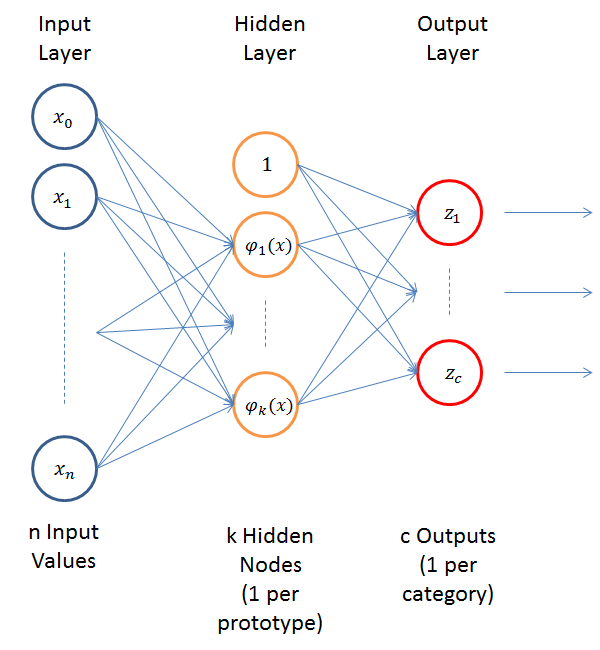
\includegraphics[scale=0.5]{../figures/nnstruct.png}
 \caption{Structure MLP à une couche cachée. \textbf{Source}: McCormick\cite{RBFtuto}}
 \label{structuremlp}
\end{figure}
Un \mlp est composé de plusieurs couches (Figure \ref{structuremlp}):
\begin{center}
 couche d'entrée $\rightarrow$ couches cachées $\rightarrow$ couche de sortie.
\end{center}
Un neurone envoie sa sortie vers tous les neurones de la couche suivante.
Il y a autant de neurones d'entrées que la dimension du vecteur d'entrée.
Le $k$\textsuperscript{ième} neurone d'entrée renvoie juste le $k$\textsuperscript{ième} élément du vecteur d'entrée.
Chaque neurone de sortie correspond à une dimension du vecteur de sortie.
Les neurones cachés et neurones de sortie correspondent à la Figure \ref{neuronemlp}.
\subsubsection{Apprentissage supervisé}\label{sec:appmlp}
Il existe plusieurs algorithmes pour changer les poids sur un réseau. Mais le plus connu est l'algorithme de de rétropropagation.\cite{Haykin,Gauthier}
Il s'agit d'un algorithme d'\emph{apprentissage supervisé}.
\begin{definition}
L'apprentissage supervisé est une méthode visant à améliorer un approximateur grâce à un calcul d'erreur (appelé aussi mesure de performance\cite{Gauthier}) comparant une sortie générée avec la sortie attendue.
\end{definition}
Nous avons donc besoin d'un ensemble de paires d'entrées/sorties.
L'algorithme applique la formule développée ci-dessous à tous les neurones sauf les neurones d'entrée.\\

Soit $\phi$, la fonction d'activation. Soit $\phi'$ la dérivée de $\phi$. Soit $Q$ l'\emph{erreur quadratique} utilisé comme mesure de performance.
\[Q = \frac{1}{2}\sum_{i}(\phi_i-s_i)^2\] où $\phi_i$ est la sortie du neurone de sortie $i$ et $s_i$ la sortie attendue pour la dimension $i$.
La modification du poid $W_{ij}$ vaut \[\Delta W_{ij} = -\eta\partiel{Q}{W_{ij}}\] où $\eta$ est une constante appelé \emph{pas du gradient}.
Par le théorème de dérivation des fonctions composées, \[\partiel{Q}{W_{ij}} = \partiel{Q}{\phi_i} \partiel{\phi_i}{v_i} \partiel{v_i}{W_{ij}}\]
\begin{thm}[dérivation des fonctions composées]
Soit $f:A~\rightarrow~B : y~\rightarrow~f(y)$ et $g:B~\rightarrow~C : x~\rightarrow~g(x)$. Alors la dérivée de $f~\circ~g$ en $x$ vaut
\[\partiel{f}{x} = \partiel{f}{g} \partiel{g}{x}\]
\end{thm}
Posons $\delta_i = \partiel{Q}{\phi_i} \partiel{\phi_i}{v_i}$. $\delta_i$ est appelé \emph{contridution à l'erreur} du neurone $i$ et est utilisé pour l'apprentissage des neurones de la couche prédédente.
Ensuite, soit $x_i$ l'entrée du neurone $i$,
\begin{equation}
 \begin{split}
  \partiel{v_i}{W_{ij}} & = \partiel{(W_{i0}x_i)}{W_{ij}} + \partiel{(W_{i1}x_i)}{W_{ij}} + ... + \partiel{(W_{ij}x_i)}{W_{ij}} + ... + \partiel{(W_{im}x_m)}{W_{ij}}\\
  ~ & = x_i
  \end{split}
\end{equation}
On a donc \[\Delta W_{ij} = -\eta \delta_i x_i\].
Déterminons la valeur de $\delta_i$.\\

\textbf{Si le neurone $i$ est un neurone de sortie,}
Soit $m$ la dimension de l'entrée $x$ (du neurone). Soit $l$ la dimension du vecteur de sortie du réseau.
\begin{equation}
 \begin{split}
  \partiel{Q}{\phi_i} & = \frac{1}{2} \left( \partiel{(\phi_0 - s_0)^2}{\phi_i} + \partiel{(\phi_1 - s_1)^2}{\phi_i} + ... + \partiel{(\phi_i - s_i)^2}{\phi_i} + ... + \partiel{(\phi_l - s_l)^2}{\phi_i} \right)\\
  ~ & = \frac{1}{2}2(\phi_i - s_i)\partiel{(\phi_i - s_i)}{\phi_i}\\
  ~ & = (\phi_i - s_i) 1\\
  \partiel{\phi_i}{v_i} & = \phi'(v_i)
 \end{split}
\end{equation}\label{eq:a}
On obtient donc \[\delta_i = (\phi_i - s_i)\phi'(v_i)\]\\

\textbf{Si le neurone $i$ est un neurone caché,}
Soit $m$ la dimension de l'entrée $x$ (du neurone). Soit $n$ le nombre de neurone de la couche suivante.
L'indice $k$ sera utilisé pour désigner un neurone de la couche suivante.
\begin{equation}
 \begin{split}
  \partiel{Q}{\phi_i} & = \sum_{k=1}^{n} \partiel{Q}{\phi_k} \partiel{\phi_k}{v_k} \partiel{v_k}{\phi_i}\\
  ~ & = \sum_{k=1}^{n} \delta_k \partiel{v_k}{\phi_i}
 \end{split}
\end{equation}
Or $\phi_i$ est l'entrée du neurone $k$ recevant la sortie du neurone $i$. Posons $W_{ki}$ le poid que $k$ attribue à $\phi_i$.
On obtient donc \[\partiel{v_k}{\phi_i} = \partiel{W_{ki}\phi_i}{\phi_i} = W_{ki}\]
Comme pour les neurones de sorties, $\partiel{\phi_i}{v_i} = \phi_i'(v_i)$.
Et du coup, \[\delta_i = \phi_i'(v_i) \sum_{k=1}^{n} \delta_k W_{ki}\]
\subsubsection{Apprentissage non supervisé}
Il existe également des algorithmes d'apprentissage non supervisé.
Ces algorithmes ne cherche pas à minimiser une erreur mais maximisent un score calculé à partir de la sortie du réseau.
\subsubsection{Apprentissage sur plusieurs MLP}
Lorque l'une des dimensions du vecteur d'entrée est discrète et finie, il est conseillé d'utiliser un \mlp différent par valeur différente sur cette dimension.\cite{Gauthier}
Cette technique peut aussi être utilisé si nous pouvons classer tous les états possibles selon le contexte.
Par exemple, pour la Sphero nous pourrions utiliser un \mlp pour le contexte \enum{en train de déraper} et un autre \mlp pour le contexte \enum{ne dérape pas}.
\subsubsection{Applications}
À une couche cachée, un \mlp peut déja servir pour la classification non linéaire.\cite{statistica}\\
Les \mlp sont aussi utilisés en commande de robot par caméra.\cite{Pomerleau}
\subsection{Fonctions à base radiale}
Nous désignerons un réseau de neurones \emph{fonctions à base radiale} par sa terminologie anglaise: \rbf pour \enum{Rasial Basis Function}.
\newcommand{\factnorm}{\sum_{r=1}^{m}x_{r}}
\subsubsection{Neurone}
Un neurone \textbf{caché} d'un \rbf n'effectue pas de somme pondérée de ses entrées.
Il applique directement sa fonction d'activation $\phi$, une gaussienne de moyenne $\mu$ et d'écart-type $\sigma$ où $x$, de dimension $n$, est l'entrée du neurone.
\begin{equation}\label{eq:cachephi}
 \phi(x) = e^{-\frac{1}{2}\sum_{k=1}^{n}\frac{(x_k-\mu_{ik})^2}{\sigma_{ik}^{2}}}
\end{equation}
Où $i$ est l'indice du neurone. $\mu$ s'appelle aussi \emph{prototype} dans le cas d'un \rbf.
%$\phi(x)$ peut se résumer en: \[\phi(x) = e^{-\beta||x-\mu||^2}\]Où $\beta$ est donc un coefficient qui règle la largeur de la courbe en cloche.\\
\\

Un neurone \textbf{de sortie} d'un \rbf n'effectue pas non plus de somme pondérée de ses entrées. Sa fonction d'activation est:
À une couche cachée, un \mlp peut déja servir pour la classification non linéaire.\cite{statistica}\\
\begin{equation}\label{eq:sortiephi}
 \phi(x) = \frac{\sum_{j=1}^{m}W_{ij}x_{j}}{\sum_{j=1}^{m}x_{j}}
\end{equation}
Où $i$ est l'indice du neurone et $x$ l'entrée de dimension $m$.
\begin{figure}
 \centering
 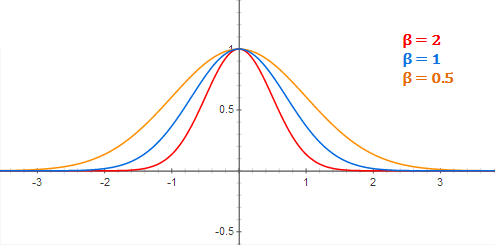
\includegraphics[scale=0.7]{../figures/RBFactivation.png}%TODO generer ça soit-même
 \caption{Activation d'un neurone RBF avec différentes valeurs d'écart-type}
 \label{rbfactivation}
\end{figure}
La Figure \ref{rbfactivation} représente la sortie d'un neurone \rbf où $\mu$ et $x$ sont de dimension 1 et $\mu = 0$.\\
Pour résumer, un neurone \rbf renvoie une valeur indiquant la simularité entre l'entrée et son prototype.
\subsubsection{Structure}
\begin{figure}
 \centering
 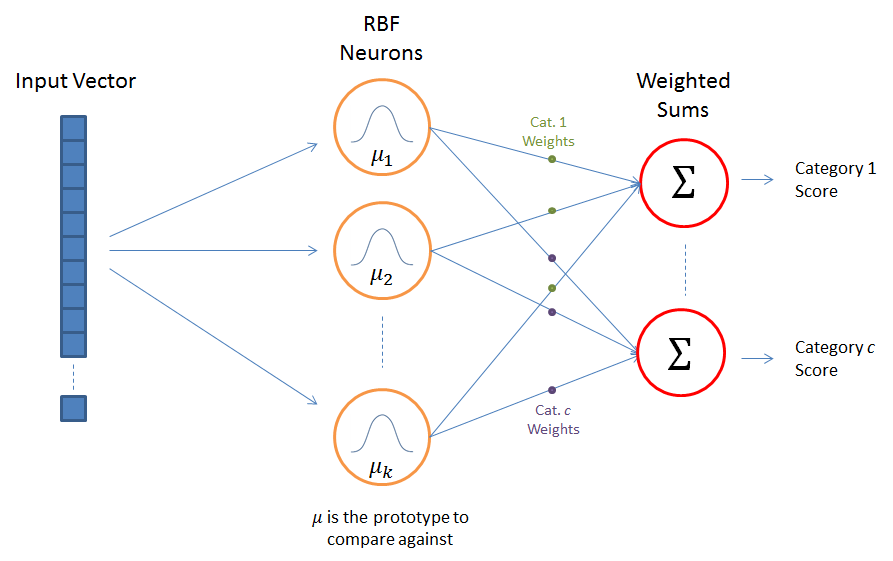
\includegraphics[scale=0.5]{../figures/RBFstruct.png}
 \caption{Structure RBF. \textbf{Source}: McCormick\cite{RBFtuto}}
 \label{structurerbf}
\end{figure}
La structure d'un \rbf est comme celle du \mlp sauf qu'il n'y a qu'une seule couche cachée (Figure \ref{structurerbf}).
\subsubsection{Apprentissage}
Dans ce réseau, les paramètres qui seront modifiés lors de l'apprentissage sont les poids des neurones de sortie et les moyennes et écart-types des neurones cachés.
L'algorithme de rétropropagation peut être utilisé pour un apprentissage supervisé d'un \rbf.
Reprenons \eqref{eq:Q}, l'erreur quadratique $Q$ défini dans la section \ref{sec:appmlp}.
En reprenant le même raisonnement que la rétropropagation dans un \mlp,
on va faire un pas de $\eta$ dans le sens opposé et proportionnel au gradient pour chaque poid $W_{ij}$ des neurones de sortie mais aussi des prototypes $\mu_i$ et écart-types $\sigma_i$ des neurones cachés.
C'est à dire que les paramètres seront modifiés de la sorte:
\begin{equation}%\label{eq:modifpoid}
 \Delta W_{ij} = -\eta \partiel{Q}{W_{ij}}
\end{equation}
\begin{equation}%\label{eq:modifmu}
 \Delta \mu_{ik} = -\eta \partiel{Q}{\mu_{ik}}
\end{equation}
\begin{equation}%\label{eq:modifsigma}
 \Delta \sigma_{ik} = \eta \partiel{Q}{\sigma_{ik}}
\end{equation}

Le dévellopement des formules de rétropropagation a été fait en annexe \ref{sec:eqrbf}.
Et voici ce que nous obtenons au final:\\
Pour un neurone de sortie :
\[\Delta W_{ij} = -\eta (\phi_i - s_i) \frac{x_j}{\factnorm}\]
Pour un neurone caché, posons $x_r$ l'entrée de $j$ provenant de $i$ (c'est à dire $\phi_i = x_r$),\\
posons $n$ la dimension de l'entrée de $j$,\\
posons aussi $R = \sum_{k=1}^{n}x_k$.
\[\Delta\mu_{ik} = -\eta \left[\sum_{i}(\phi_j - s_j) \frac{1}{R^2} \left(W_{jr}R - \sum_{k=1}^{n}W_{jk}x_k\right)\right] \phi_i\frac{x_k-\mu_{ik}}{\sigma_{ik}^2}\]
\[\Delta \sigma_{ik} = -\eta \left[\sum_{i}(\phi_j - s_j) \frac{1}{R^2} \left(W_{jr}R - \sum_{k=1}^{n}W_{jk}x_k\right)\right] \phi_i \frac{(x_k-\mu_{ik})^2}{\sigma_{ik}^3}\]

\subsubsection{Applications}
Un \rbf peut aussi servir pour la commande de robot.\cite{Gauthier}

Un des inconvénients des \rbf est que le nombre de neurones cachés croît avec la dimension et la taille du vecteur d'entrée puisqu'un neurone caché s'active seulement pour des entrées dans le voisinage de son prototype.
Nous pouvons raisonablement envisager ce modèle pour notre application puisque la description de l'état actuel et de l'état cible contiendra typiquement une coordonnée, un vecteur vitesse, une orientation et éventuellement l'accéleration, etc...
La taille de l'entrée sera donc relativement petite. Ce sera lors de la phase pratique qu'on évaluera le nombre de neurones cachés nécessaires.
De plus, les \rbf sont moins sensibles au bruit.\cite{adversarial}
%\subsection{Convolutif (CNN)}
\subsubsection{Réseau de neurones récurrent (RNN)}
Jusque maintenant, nous avons vu des réseaux de neurones \emph{feedforward}.
C'est à dire qu'ils ne présentent aucune boucle. Mais il éxiste des réseaux de neurones présentant des boucles.
Cela leur permet de prendre en compte les entrées précédentes.
\ssstitle{Structure}
\begin{figure}
 \centering
 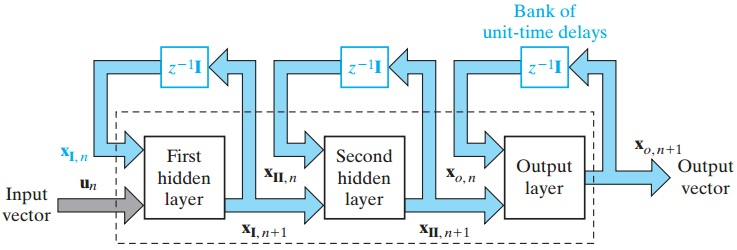
\includegraphics[scale=0.5]{../figures/structurermlp.jpg}
 \caption{Structure RLMP. \textbf{Source}: Haykin. p795\cite{Haykin}}
 \label{structurermlp}
\end{figure}
\begin{figure}
 \centering
 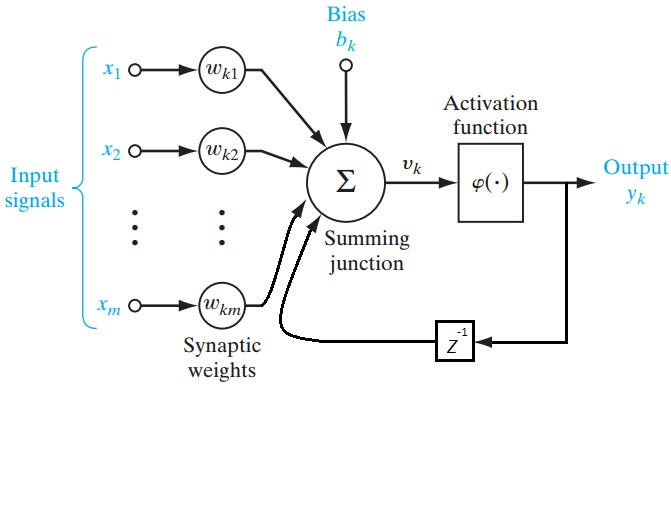
\includegraphics[scale=0.5]{../figures/neuronermlp.jpg}
 \caption{Neurone caché d'un RMLP}
 \label{neuronermlp}
\end{figure}
Un réseau de neurones récurrent est un réseaux présentant des boucles dans sa structure.
Des \emph{délais} notés $Z^{-1}$ sont présents sur certains arcs dans le réseau afin de retarder d'une étape, la transmission d'une valeur.
Une étape dans un réseau consiste à recevoir une entrée et de générer une sortie.
Il existe plusieurs réseaux de type récurrent (récurrent simple, machine à états liquide, etc).
La Figure \ref{structurermlp} présente un réseau de type perceptron multi-couches récurrent (\rmlp).
Il s'agit d'un \mlp dont les neurones des couches cachées ont un arc qui boucle sur le neurone lui-même avec un $Z^{-1}$ sur cet arc, comme sur la Figure \ref{neuronermlp}.
\ssstitle{Applications}
Grâce aux délais, le réseau peut approximer des fonctions dont la sortie ne dépend pas seulement de l'entrée actuelle mais aussi des entrées précédentes.
Mais cette fonctionnalité n'est pas utile pour notre application puisque les commandes à générer ne dépendent pas des états précédents l'état actuel.
%Les \emph{machines à états liquides} (\lsm), dont les connections se font de manière aléàtoire, sont utilisés pour la reconnaissance automatique de la parole. %TODO citer
%Les \emph{long-short term memory} sont utilisés pour la reconnaissance automatique de la parole ou de l'écriture manuscrite. %TODO citer
%\subsection{CMAC}

\section{Surajustement}
\subsection{Le phénomène}
Lorsque un réseau de neurones à apprentissage supervisée apprend de trop nombreuses fois à partir du même set d'exemple, alors il se produit un phénomène appelé \emph{surajustement}.\cite{statistica}
Le réseau devient dès lors de moins en moins éfficace sur des entrées non rencontrées pendant les phases d'apprentissage.
Sur la Figure \ref{interruption}, on voit que au fil des cycles d'apprentissages (un cycle = un apprentissage sur toutes les paires entrée/sortie), l'erreur diminue.
Mais à un certain cycle, l'erreur sur des paires entrée/sortie non fournies pendant le test d'apprentissage augmente.
C'est à partir de là que le réseau de neurones surajuste.
\begin{figure}
 \centering
 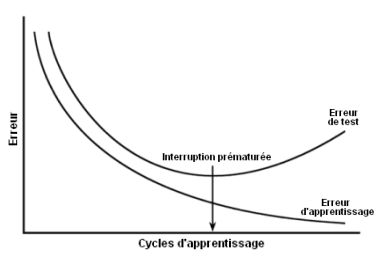
\includegraphics[scale=0.6]{../figures/surgeneralisation.jpg}
 \caption{Interruption prématurée. \textbf{Source}: STATISTICA Réseaux de Neurones Automatisés (SANN)\cite{statistica}}
 \label{interruption}
\end{figure}
\subsection{Les solutions}
\subsubsection*{Intérruption prématurée}
Tout d'abord séparons notre ensemble de paires entrée/sortie en deux ensembles.
L'un est nommé \emph{ensemble d'apprentissage} et l'autre \emph{ensemble de test}.
Chacun de ces ensembles doit balayer toutes la valeurs de vecteur d'entrée possibles.
Ensuite à chaque cycle, on va d'abord effectuer un apprentissage pour chaque paires de l'ensemble de test.
Puis on génère des sorties à partir des entrées de l'ensemble de test.
On compare l'erreur de test, c'est à dire l'erreur sur les sorties générées et les sorties attendues de l'ensemble de test, à l'erreur de test du cycle précédent.
Si l'erreur de test est plus grand que celui du cycle précédent, alors on arrête les cycles d'apprentissage.
Dans la Figure \ref{interruption}, on observe que l'intérruption prématurée se produit au moment où son \emph{pouvoir de généralisation} est le plus élevé.
C'est à dire l'éfficacité du réseau sur des entrées jamais rencontrées.\\

Attention, dans la réalité, la courbe d'erreur de test n'est pas aussi lisse que dans la Figure \ref{interruption} mais présente un certain bruitage.
Il faut donc pouvoir s'assurer que l'intérruption prématurée a bien lieu sur le minimum global de l'erreur de test.
Comparer l'erreur de test à celui du cycle précédent permet juste de détecter un minimum local.
\subsubsection*{Modération des poids}
Cette méthode consiste à pénaliser l'utilisation de trop grand poids.
Pour ce faire, on modifie le calcul d'erreur pour y prendre en compte la valeur des poids.\cite{statistica}
Soit $E$ l'erreur, soit $W$ un vecteur contenant tous les poids (ne pas prendre les biais en compte), la nouvelle valeur de l'erreur est \[E_{new} = E + \frac{\sigma}{2}W^{T}W\]
Où $\sigma$ est une constante appelé \emph{constante de modération}.
Un $\sigma$ trop petit ne permet pas d'éviter le surajustement et un $\sigma$ trop grand empêche la généralisation.

\section{Méthodes d'apprentissage avec maître distant}
Nous allons observer différentes architectures intéressantes dans le cas de génération de commandes.
Le mot \enum{architecture} utilisé ici ne désigne pas l'architecture d'un réseau de neurones mais l'architecture d'une méthode d'utilisation de réseaux de neurones.
La convention graphique est montré dans la Figure \ref{legendearchi}.
\begin{figure}
 \centering
 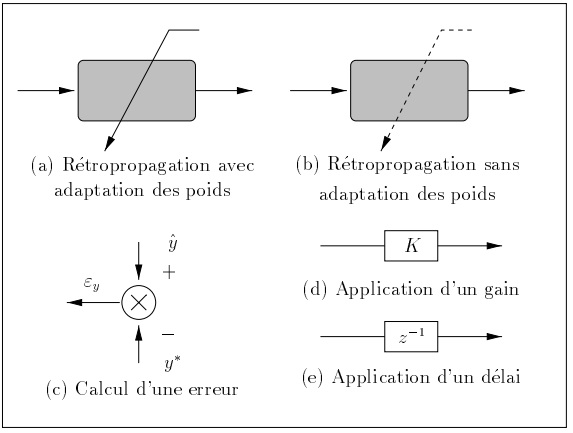
\includegraphics[scale=0.6]{../figures/applegende.jpg}
 \caption{Conventions graphiques pour la descriptions de l'architecture d'une méthode utilisant des RNA. \textbf{Source}: Gauthier\cite{Gauthier}}
 \label{legendearchi}
\end{figure}

\subsection{Le problème}
Dans cette section, nous allons voir différentes méthodes pour entrainer un réseau de neurones à générer des commandes.
Ces méthodes visent à contourner le \emph{problème de l'apprentissage avec maître distant}.
Dans l'apprentissage supervisé, un \emph{maître} est ce qui permet de fournir une erreur entre la sortie d'un réseau de neurones et la sortie attendue.
Et effectivement dans notre cas, nous n'avons rien qui puisse nous permettre de définir les commandes idéales à éxécuter pour passer d'un certain état à l'autre.
Par contre nous pouvons avoir un maître qui compare l'état résultant de l'exécution d'une commande à l'état cible.

Dans les figures qui suivront, Système désigne l'exécution, dans la réalité, de la commande entrée.
En sortie du Système nous avons l'état résultat de l'exécution des commandes.

\subsection{Reproduction d'un contrôleur}
\begin{figure}
 \centering
 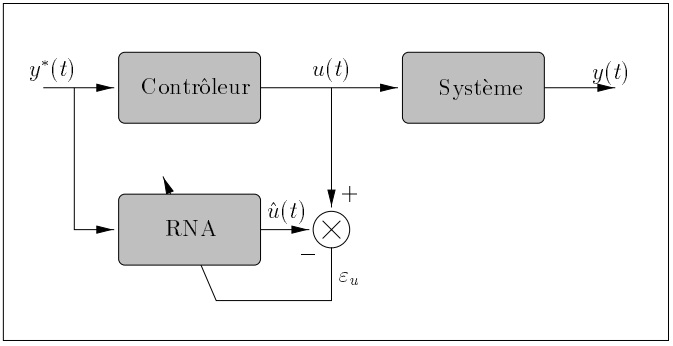
\includegraphics[scale=0.5]{../figures/appsimple.jpg}
 \caption{Apprentissage par reproduction d'un contrôleur. \textbf{Source}: Gauthier\cite{Gauthier}}
 \label{appcontroleur}
\end{figure}
Dans cette méthode d'apprentissage, le \rna apprend à reproduire les commandes d'un contrôleur existant (\textbf{Figure \ref{appcontroleur}}).
Cette méthode a été utilisé pour commander le volant d'une voiture pour suivre des virages où le controlleur est un humain.\cite{Pomerleau}

\subsection{Apprentissage spécialisé}\label{sec:appspecial}
\begin{figure}
 \centering
 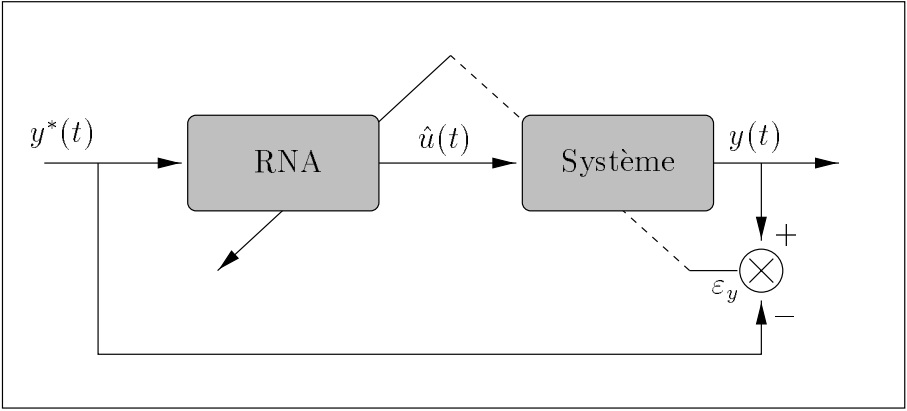
\includegraphics[scale=0.4]{../figures/appspecialise.jpg}
 \caption{Apprentissage spécialisé. \textbf{Source}: Gauthier\cite{Gauthier}}
 \label{appspecialise}
\end{figure}
Ici on applique l'algorithme de rétropropagation en démarrant depuis le maître distant et en passant par le système.
Par exemple, nous avons vu que, dans le cas d'un \mlp, section \ref{sec:appmlp}, l'apprentissage est l'application de la formule \[\Delta W_{ij} = -\eta\partiel{Q}{W_{ij}} = \partiel{Q}{\phi_i} \partiel{\phi_i}{v_i} \partiel{v_i}{W_{ij}}\]
En reprenant la notation de la Figure \ref{appspecialise}, \[\Delta W_{ij} = -\eta\partiel{\varepsilon_y}{W_{ij}} = \partiel{\varepsilon_y}{\hat{u}} \partiel{\hat{u}}{v_i} \partiel{v_i}{W_{ij}}\]
Où $v_i$ est la somme pondérée des entrées du neurones $i$.
Or $\partiel{\varepsilon_y}{\hat{u}} = \partiel{\varepsilon_y}{y}\partiel{y}{\hat{u}}$. Et donc la formule devient
\[\Delta W_{ij} = \partiel{\varepsilon_y}{y} \partiel{y}{\hat{u}} \partiel{\hat{u}}{v_i} \partiel{v_i}{W_{ij}}\]
Et définir le facteur $\partiel{y}{\hat{u}}$ est la difficulté de cette méthode:
Il faut pouvoir modèliser le système par une fonction $y(\hat{u})$ dérivable en $\hat{u}$.
%TODO et dans le cas d'un RBF ?

\subsection{Apprentissage en deux phases}\label{sec:app2phases}
\begin{figure}
 \centering
 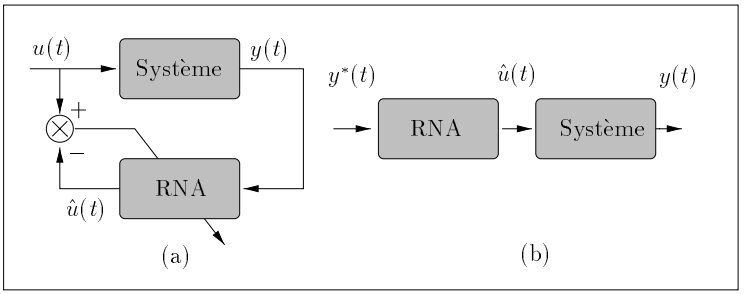
\includegraphics[scale=0.5]{../figures/app2phases.jpg}
 \caption{Apprentissage en deux phases. \textbf{Source}: Gauthier\cite{Gauthier}}
 \label{app2phases}
\end{figure}

Tout d'abord, (a) On génère des commandes $u$ en boucle et on les applique au système (\textbf{Figure \ref{app2phases}}).
Soit $y$ l'état du robot après avoir appliqué la commande $u$, on obtient en boucle des paires entrée/sortie où $y$ est l'entrée et $u$ la cible.
On continue la boucle pour balayer toutes les configurations possibles de $u$.

Puis vient la phase d'utilisation (b) où on utilise le réseau cette fois pour génèrer les commandes. Mais sans apprentissage. L'adaptabilité est donc sacrifiée.\\

Cette méthode est inadapté dans les cas où il existe plusieurs commandes idéales pour un même état cible.
En effet, imaginons qu'il existe deux commandes idéales pour atteindre le même état cible et que ces deux commandes soient rencontrées lors de la phase (a).
Alors les poids seront modifiés pour que la sortie converge vers la première commande idéale rencontrée, puis l'autre et ainsi de suite.
Et finalement, la sortie du réseau pour cet état cible ne va pas converger vers une des commandes idéales.

\subsection{Apprentissage indirecte}\label{sec:appindirect}
\begin{figure}
 \centering
 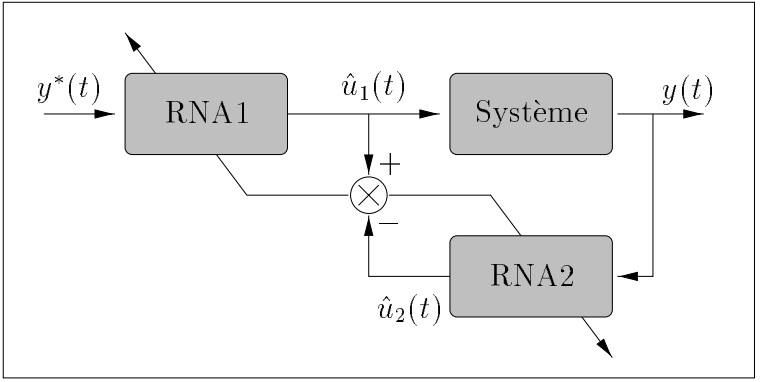
\includegraphics[scale=0.5]{../figures/appindirect.jpg}
 \caption{Apprentissage indirect. \textbf{Source}: Gauthier\cite{Gauthier}}
 \label{appindirect}
\end{figure}
L'apprentissage indirecte, montré dans la \textbf{Figure \ref{appindirect}}, est une méthode qui permet de retrouver l'adaptabilité. (sacrifiée dans l'apprentissage en deux phases, section \ref{app2phases})
RNA1 et RNA2 ne sont pas deux réseaux différents. Il s'agit du même réseau de neurones.
RNA1 et RNA2 partagent les mêmes poids.
Mais selon Gauthier\cite{Gauthier}, cette méthode tend à toujours donner la même commande.

\subsection{Apprentissage par modèle différentiable}\label{sec:appmodele}
\begin{figure}
 \centering
 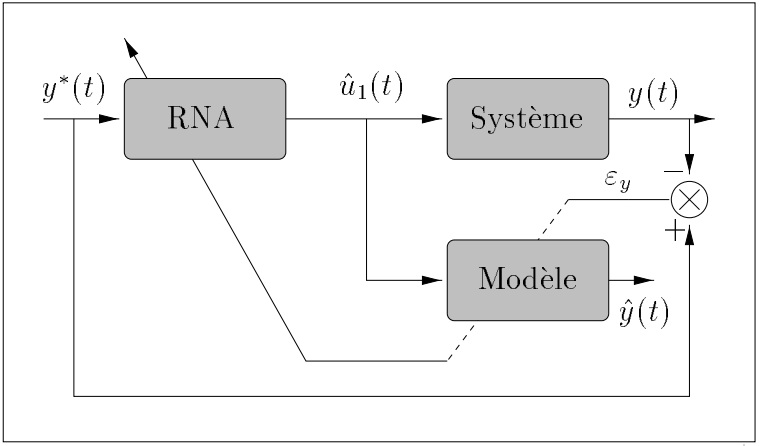
\includegraphics[scale=0.5]{../figures/modelediferentiable.jpg}
 \caption{Apprentissage par modèle différentiable. \textbf{Source}: Gauthier\cite{Gauthier}}
 \label{appmodele}
\end{figure}

L'idée est d'utiliser la méthode de l'apprentissage spécialisé à la section \ref{sec:appspecial} mais en se servant d'un \rna comme modèle différentiable (\textbf{Figure \ref{appindirect}}).
Il faut donc, dans un premier temps, établir un \rna qui va apprendre à prédire le prochain état selon la commande à exécuter.
Nous n'avons pas le problème de l'apprentissage avec maître distant pour ce \rna car sa sortie peut directement être comparée à la sortie du système.
Ensuite, on l'utilise comme modèle. Et là nous pouvons connaître $\partiel{\varepsilon_y}{\hat{u}_1}$ grâce aux formule de rétropropagation de la section \ref{sec:appmlp}.\\
%TODO prouver et parler aussi de formule de backpropagation pour rbf

L'adaptabilité est sacrifiée car si le système change et que le modèle n'a pas été entrainé pour ce nouveau système, l'algorithme de rétropropagation va faire converger la solution vers des commandes inadaptés pour le nouveau système.

\subsection{Apprentissage sur plusieurs étapes}
Un autre problème qui peut se présenter pour la commande par réseaux de neurones est d'obtenir un maître distant seulement après plusieurs étapes.
Par exemple, imaginons que nous voulons commander la marche d'un robot avec un réseau de neurones qui fournira des commandes tous les $T$ secondes.
Si le robot tombe et que nous pouvons en obtenir un maître, nous ne savons pas à quelles étapes avant la chute le réseau a fourni des commandes responsables de cette chute.\\

Une solution à ce problème est l'architecture de Nguyen et Widrow, Figure \ref{appNguyenWidrow}.
\begin{figure}
 \centering
 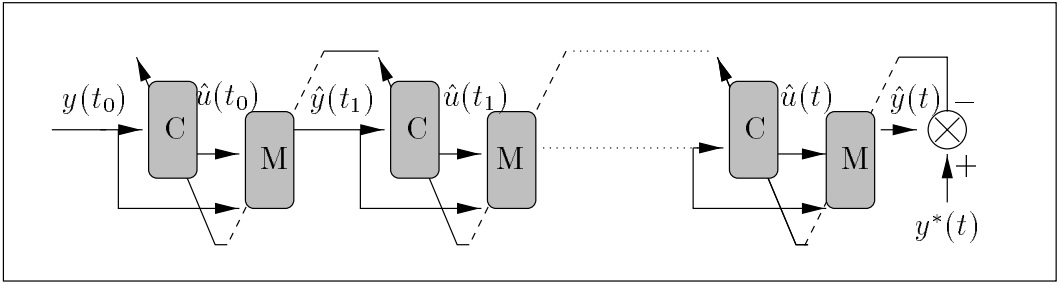
\includegraphics[scale=0.5]{../figures/appNguyenWidrow.jpg}
 \begin{itemize}
  \item \textbf{C}: Réseau qui génère les commandes
  \item \textbf{M}: Modèle
 \end{itemize}
 \caption{Architecture de Nguyen et Widrow. \textbf{Source}: Gauthier\cite{Gauthier}}
 \label{appNguyenWidrow}
\end{figure}
Cela consiste à utiliser un modèle différentiable (qui peut être un réseau de neurone) pour pouvoir effectuer l'algorithme de rétropropagation jusque la première étape après l'obtention du maître précédent.

\newpage
\section{Implémentation et application}

\subsection{Design du vecteur d'entrée}
\subsubsection{Données utiles}
Avant de choisir le réseau de neurones à utiliser pour Générer des commandes pour la Sphero, il est important d'identifier ce que nous souhaitons obtenir en sortie et les informations que nous pouvons fournir en entrée en omettant les données inutiles.
Si le vecteur d'entrée est de dimension très grande, alors un réseau \rbf devra avoir un trop grand nombre de neurones cachés\cite{Gauthier}.
Si nous supposons que la sortie produite peut dépendre non seulement de l'input actuel mais aussi des entrées précédentes, alors un réseau récurrent devra être utilisé.

La Sphero peut nous fournir:\cite{SDKofficiels}
\begin{itemize}
 \item Sa position grâce à un odomètre (cm),
 \item Son vecteur vitesse (mm/s),
 \item Son vecteur d'accélération grâce à un accéleromètre (mG),
 \item Son orientation (-179$\rightarrow$180 degrés),
 \item Son niveau de charge (Pas de poucentage mais label \enum{Chargement}, \enum{OK}, \enum{Bas} et \enum{Critique}),
 \item État des LEDs, évènement de collision, voltage de la batterie, nombre de charges, version ...
\end{itemize}

Parmis ces données, nous n'avons pas besoin de l'état des LEDs, version et nombre de charges car ils n'influencent pas la conduite de la Shero.
Dans ce projet, nous ne prenons pas en compte les éventuels collisions.

Le niveau de charge pourrait influencer la conduite.
Nous ne savons pas si la puissance maximale des moteurs diminuent lorsque la charge est trop faible.
Si cela s'avère être le cas, pour ne pas devoir effectuer un entrainement pour chaque niveau de charge différent, on entrainera la Sphero que pour les cas où le niveau de charge est à \enum{OK} et on supposera donc que la conduite sera effectuée qu'avec ce niveau de charge.

Un odomètre n'est pas approprié pour la mesure de position dans notre application.
En effet, la distance parcourue n'est mesurée qu'à partir du roulement du moteur permettant le déplacement.
La distance parcourue par dérapage ne sera pas comptabilisée.
Cela a été vérifié lors de l'expérience menée dans la section \ref{sec:choixdesign}.
Une camera sera utilisée pour tracer la position réelle de la Sphero.

Pour l'accélération, les commandes à appliquer à l'instant $t$ ne dépendent pas de l'accélération à l'instant $t$ juste avant l'application des commandes.
Mais par contre, cette donnée peut être utile pour anticiper la vitesse de la Sphero au moment où elle reçoit les commandes car du à la latence d'envoi de paquet, la vitesse à l'instant $t$ n'est plus la même que celle communiquée.
Si cette donnée impacte peu dans les résultats obtenus, alors nous pourrions décider de nous passer de ce paramètre.
Ajouter cette dimension dans le vecteur d'entrée demandera un plus grand nombre d'exemples pour la phases d'apprentissage car il faut balayer toutes les configurations possibles de vecteur d'entrée.

\newcommand{\inchist}[1]{
 \begin{minipage}{0.48\textwidth}
  \includegraphics[width=10cm]{../figures/hist#1.jpeg}
 \end{minipage}
}
\subsubsection{Choix du design}\label{sec:choixdesign}
 %TODO montrer les design repris chez gauthier
Pour une meilleure précision, on ajoute un vecteur vitesse à atteindre sur le point de destination.
On aligne l'axe des abscisses avec l'axe de l'orientation du moteur afin de reduire le domaine d'entrée et donc le nombre d'exemples à créer pour l'apprentissage.
Le vecteur d'entrée contiendra donc le vecteur vitesse, la position relative à atteindre dans $T$ secondes où $T$ sera la période à laquelle on échantillonera les données des capteurs.
Nous avons donc un vecteur d'entrée à 6 dimensions (vitesse actuelle en x et y, position relative cible en x et y, vitesse cible en x et y).
Le vecteur de sortie sera la puissance à donner pour chaque moteur.

Estimons la valeur optimale que nous pouvons donner à $T$.
Une commande de streaming de donnée peut être envoyée à la Sphero.
Grâce à cette commande, nous pouvons demander à la Sphero d'envoyer uniquement les données qui nous interessent à une fréquence donnée.
Trois paramètres de cette commande peuvent influencer les performances d'échantillonage:
\begin{enumerate}
 \item Un diviseur (entier) de la fréquence maximale d'échantillonage.
 \item Le nombre d'échantillonage à garder en mémoire avant envoi.
 \item Le nombre de capteur à échantilloner.
\end{enumerate}
Un échantillonage consiste à obtenir seulement les données qui nous intéressent à un instant précis.
La fréquence maximale d'échantillonage, un échantillon à la fois, est de 400Hz.\cite{SDKofficiels}
La vitesse maximale de la Sphero est de 4,5 miles par heure.\cite{product} Ce qui fait environ 2 mètres par seconde.
\begin{figure}
 \centering
 \inchist{20}
 \inchist{40}
 \inchist{60}
 \inchist{80}
 \inchist{100}
 \inchist{200}
 \caption{Histogrammes de temps de réception de packet streamé. Générés via script R}
 \label{histogrammes}
\end{figure}

À la Figure \ref{histogrammes} sont repris les histogrammes de temps de réceptions de paquets pour différentes fréquences d'échantillonage.
En plus du streaming, pour chaque paquet reçu, un paquet est envoyé à la Sphero pour changer les leds.
Cela nous permet d'obtenir des résultats qui se rapprocheront de ce que nous obtiendrons si nous envoyons une nouvelle commande à chaque période $T$.
La configuration de l'ordinateur utilisé est la suivante:
\begin{itemize}
 \item AMD Athlon(tm) X2 Dual-Core QL-64
 \item Carte mère EI Capitan
 \item 3 Go de RAM DDR2
 \item disque dur ST9250827AS 5400rpm
 \item Adapteur USB bluetooth BT009x, transfert 1Mbs.
 \item OS: Linux 4.4.0-57-generic, Ubuntu 16.04.4
\end{itemize}

On observe tout d'abord que les temps de réception ont l'air de suivre une cadence de 1ms.
Cela peut s'expliquer par le fait que la Sphero 2.0 a une granularité de 1ms pour l'éxecution de macro.\cite{product}
%Plus $T$ est petit, plus notre système de commande est réactif et, toutes choses égales par ailleur, nous pouvons effectuer des mouvements plus précis.
Pour les critères de choix d'une valeur pour $T$, deux critères sont pris en compte:
\begin{enumerate}
 \item La stabilité du streaming. Moins la densité de probabilité de temps de réception de paquet est concentrée sur le voisinage de $T$, moins la solutions sera précise.
 \item Le temps de réaction. Plus $T$ est grand, moins la trajectoire de la Sphero sera fidèle à la trajectoire voulue.
 Nous pouvons compenser ce manque de précision par un vecteur d'entrée plus complexe mais la solution converge alors moins vite et un ensemble d'apprentissage plus conséquent doit être fournis.
\end{enumerate}

On observe que la stabilité du streaming varie selon la fréquence.
Prenons le streaming à 60Hz. On observe que en moyenne les paquets arrivent toutes les 15 millisecondes.
La distance maximale que peut parcourir la Sphero en 15ms est de 3 cm.
Le manque de précision dû au temps de réaction est dans ce cas négligeable pour des trajectoires à grande vitesse de l'ordre de quelque mètres.
De plus, ce streaming étant le plus stable, c'est cette fréquence qui sera utilisée.
Nous considèrerons donc que $T$ = 15ms malgré que la fréquence est règlée à 60Hz.


\subsection{Choix du réseau}
%TODO Tableau de comparaison
Nous n'avons pas besoin d'un réseau de neurones récurrent.
Les commandes à appliquer ne dépendent pas de la vitesse, position et autres données fournies aux étapes précédentes.
Le réseau le mieux adapté pour notre problème est un réseau de neurones à base radial.
En effet, les \rbf sont moins sensibles au bruit que les \mlp \cite{adversarial,Gauthier}.%gauthier p 39,40
Car dans la couche cachée, chaque neurone envoit une sortie indiquant la proximité entre le vecteur d'entrée et son prototype.
Donc typiquement, la contribution à l'erreur est presque entièrement celle du neurone ayant son prototype le plus proche de l'entrée.
Les autres neurones cachés auront une modification insignifiante de l'écart-type et du prototype.\\

Un des inconvénients des \rbf est que le nombre de neurones cachés croît avec la dimension et la taille du vecteur d'entrée.
Ceci ne pose pas de problème dans notre cas car le nombre de dimensions est faible.

\subsection{Choix de la méthode}
Vu toutes les inconnues mécaniques du mouvement de la Sphero, il s'avère difficile d'établir une équation permettant de prédire de manière précise l'état suivant en fonction des commandes exécutées.
Nous préfèrons donc nous passer d'un modèle analytique.
Dans ce cas, nous ne pouvons pas utiliser la méthode de l'apprentissage spécialisé.
De plus, télécommander une Sphero pour suivre une trajectoire est très difficile pour un humain.
Utiliser un apprentissage par reproduction de contrôleur n'est donc pas envisageable.\\
Nous pouvons obtenir un maître distant à chaque étape et donc nous n'avons pas besoin de l'architecture de Nguyen et Widrow.\\
Le problème de convergence vers une solution triviale, impliqué dans le cas d'un apprentissage indirect (section \ref{sec:appindirect}) exclu l'utilisation de cette méthode dans le cadre de ce projet.\\

Il nous reste deux méthodes pour lesquelles l'adaptabilité est sacrifiée: l'apprentissage en deux phases et apprentissage utilisant un modèle différentiable.
Les deux sont envisageables. Les tests seront effectués toujours sur le même sol horizontal.\\

La méthode avec modèle différentiable apportera un nouveau facteur influençant la réussite du projet: la fiabilité du modèle.
Mais puisque le sytème ne change pas, lorsqu'on arrive à obtenir un modèle fiable, nous pouvons effectuer un apprentissage en-ligne qui permettra à la Sphero de parfaire le suivi d'une trajectoire si cette trajectoire est ammenée à être répétée.
Nous utiliserons dans un premier temps la méthode en deux phases pour obtenir un ensemble de paires cible/commande où la précision dépend seulement des capteurs et pas de la fiabilité d'un modèle.

\subsection{Les API}
Certaines API permettant l'envoi de commande et réception de message provenant de la Sphero sont disponibles.
Les APIs officiels sont disponibles en: \textbf{Objective-C}, \textbf{Swift}, \textbf{Android}.\cite{SDKofficiels}\\
Il existe également des APIs créés par la communauté disponibles en\cite{gosphero}: \textbf{C\#}, \textbf{JavaScript}, \textbf{Ruby}, \textbf{Python}\cite{pythonAPI}, \textbf{Arduino}, \textbf{C++}\cite{cppAPI}.\\
L'API choisie est l'API \textbf{C++} pour le langage de programmation connu et performant exécutable sur PC.
Malgré les apparences, cet API n'est pas modulaire concernant le streaming.
En effet, le streaming est démarré dès la connection de la Sphero et la lecture des messages de streaming récupérés ne fonctionne que pour le streaming configuré pour l'application que l'auteur voulait en faire.
C'est à dire que des accès à la mémoire se font sans considération des données demandées pour le streaming et ne permet donc que de récupérer la position et la vitesse.
De plus l'écoute des messages de streaming sont non bloquants car ils sont effectués dans un thread à part.
Il n'est donc pas possible, sans modifier l'API, d'utiliser les données reçues dès leur réception.
L'API a donc été modifiée pour récupérer les données qui nous intéressent dans le cadre de ce projet mais aussi pour effectuer le design pattern observer  et le faire hériter d'une interface d'objet capable de streamer.
(Voir la section \ref{sec:impcommander} sur l'implémentation du système de commande.)

Le langage \textbf{Qt} sera utilisé pour créer les interfaces graphiques.
Cela nous permet de créer facilement des interfaces munies de boutons, menus et fenêtres afin de tracer la trajectoire.
De plus, l'implémentation du réseau de neurones pourra être directement utilisée dans un script \textbf{Qt} puisqu'il s'agit d'une extension du c++.

L'API \textbf{Caffe} sera utilisé plus tard afin de modifier facilement l'architecture du réseau de neurones dans le module de commande sans recompilation.\cite{caffe}

\subsection{Implémentation d'un réseau de neurones}
Un \rbf a été implémenté. Bien que fonctionnel, ce n'est pas ce réseau qui est utilisé dans la version actuelle du système de commande de ce projet.
Il a néanmoins été utilisé durant la phase d'expérimentation.
\subsubsection{Propriété utilisée}
Afin d'expliquer la structure de l'implémentation du réseau de neurone, nous allons tout d'abord expliquer pourquoi l'implémentation d'un neurone est indépendant de sa position et du modèle du réseau de neurones.
Et grâce à cette propriété, nous pouvons donc connecter n'importe quelle couche de neurones avec une autre sans modifier l'implémentation.
Nous pourrions donc facilement passer à une méthode d'apprentissage par modèle différentiable (Section \ref{sec:appmodele}) si cela s'avère nécessaire.
De plus, l'implémentation d'un nouveau modèle non récursif comme le \mlp nécésitera juste l'implémentation des nouveaux neurones.
En résumé, l'implémentation d'un réseau \rbf se fera à partir d'une implémentation de réseau de neurones non récursif modulaire.\\

Deux fonctions sont nécessaires pour l'implémentation d'un neurone:
\begin{enumerate}
 \item Une fonction qui permet de générer la sortie à partir de ses entrées (compute).
 \item Une fonction permettant l'apprentissage par rétropropagation (backpropagation).
\end{enumerate}
La fonction qui génère la sortie n'a besoin que des sorties des neurones de la couche précédente.
Et si on observe le développement des formules de rétropropagation dans les annexes \ref{sec:eqmlp} et \ref{sec:eqrbf},
la fonction qui permet l'apprentissage n'a besoin que de la sortie générée précédemment (cela peut être gardé en mémoire) et la \emph{contribution à l'erreur} des neurones de la couche suivante.
Le terme de contribution à l'erreur fait réference au terme $\delta$ dans la formule de modification des poids d'un \mlp (Section \ref{sec:appmlp}).
En effet, pour tous les différents neurones que nous avons vu dans ce rapport, soit $p$ un paramètre à modifier pour l'apprentissage du neurone $i$.
Soit $f_i$ la fonction appliquée aux entrées du neurone $i$ afin de générer la sortie.
$p$ doit être modifié selon la formule suivante:
\[\Delta p_i = -\eta \partiel{Q}{p_i}\]
Et afin de calculer la valeur de $\partiel{Q}{p_i}$, deux facteurs sont à connaître: $\partiel{Q}{f_i}$ et $\partiel{f_i}{p_i}$.
Pour connaître le facteur $\partiel{f_i}{p_i}$, toutes les données dont nous avons besoin se trouvent dans l'implémentation du neurone $i$ si nous y enregistrons sa sortie précédente.
Tandis que pour le facteur $\partiel{Q}{f_i}$,
si le neurone $i$ est un neurone de sortie, alors $\partiel{Q}{f_i}$ est connu, il s'agit de la dérivée partielle de l'erreur entre $f_i$ et sa valeur atendue.
Sinon $$\partiel{Q}{f_i} = \sum_{k \in \text{couche suivate}}\partiel{Q}{f_k}\partiel{f_k}{f_i}$$
Et donc $\partiel{Q}{f_i}$ peut être calculé à partir d'une implémentation dans les neurones de la couche suivante.

\subsubsection{Diagramme de classe}
\begin{figure}
 \centering
 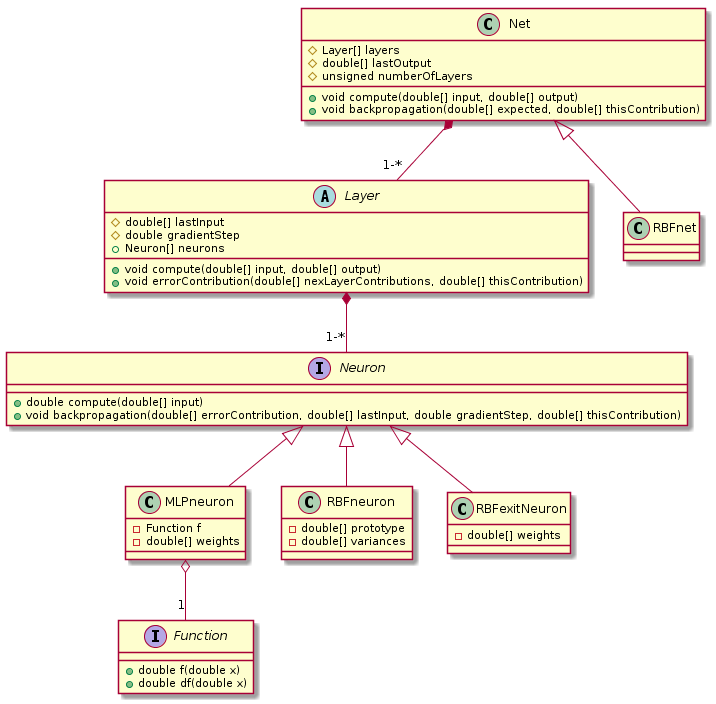
\includegraphics[width=\textwidth]{../../uml/neurondiag.png}
 \caption{Diagramme de classe du réseaux de neurones. \footnotesize Généré par \href{http://plantuml.com/class-diagram}{plantUML}}
 \label{fig:diagclasse}
\end{figure}
Dans le diagramme de classe, Figure \ref{fig:diagclasse}, dans la déclaration de la fonction \texttt{backpropagation()}, \texttt{errorContribution} est le facteur $\partiel{Q}{f_i}$.
Le tableau retourné est stocké dans \texttt{thisContribution}.
Pour chaque entrée $x_j$ du neurone $i$, la $j$\textsuperscript{ième} valeur du tableau retourné est $\partiel{Q}{f_i}\partiel{f_i}{x_j}$.
Ces valeurs sont utilisées pour effectuer la rétropropagation de la couche précédente.

\subsubsection{Limitation actuelle}
Dans la version actuelle de l'implémentation, les biais ne sont pas supportés, le MLP n'est pas encore fonctionnel et des fuites mémoires ont été détectés.
Les fuites mémoires sont dû à l'allocation de mémoire pour transmettre des valeurs d'une couche à l'autre dans \texttt{Net.cpp}.
L'opérateur \texttt{New} effectue une allocation dynamique et nécessite d'être libérée exlplicitement par le programmeur.

\subsection{Implémentation d'un système de commande}
Passons maintenant à la descriptions des différentes classes et interfaces du système de commande.

\newcommand{\classname}[1]{\textbf{\texttt{#1}}}
\subsubsection{Structure}
\begin{figure}
 \centering
 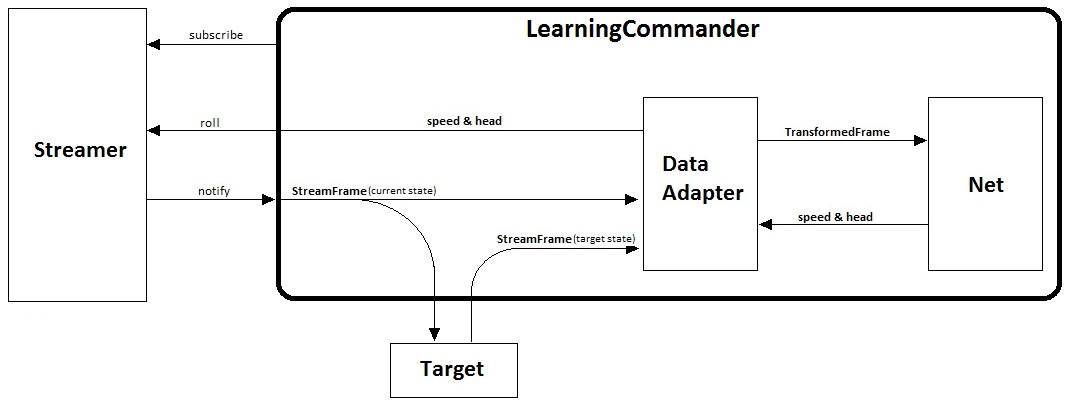
\includegraphics[width=0.8\textwidth]{../figures/commander.jpg}
 \caption{Structure du système de commande}
 \label{fig:commander}
\end{figure}
\begin{figure}
 \centering
 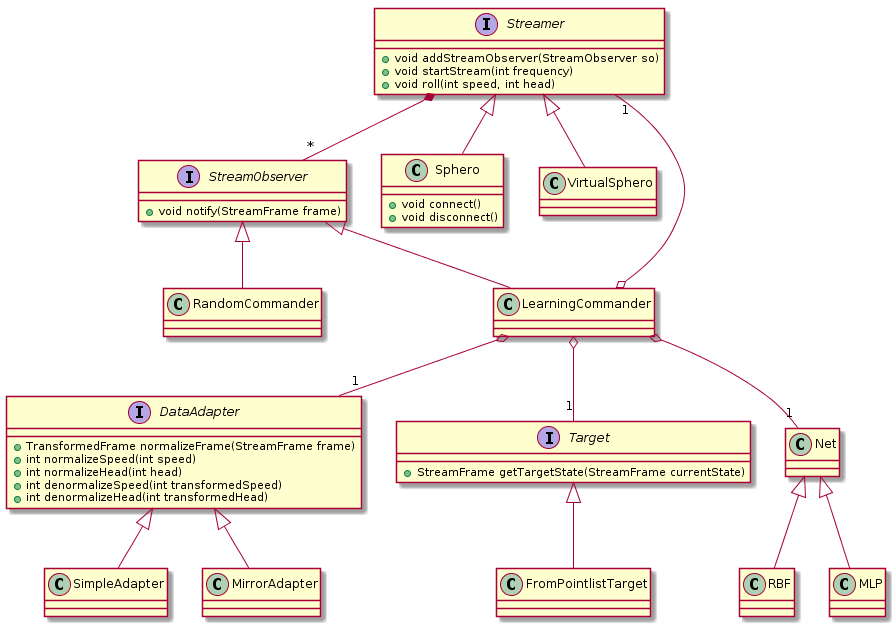
\includegraphics[width=\textwidth]{../../uml/commanderdiag.png}
 \caption{Diagramme de classe dy système de commande.\footnotesize Généré par \href{http://plantuml.com/class-diagram}{plantUML}}
 \label{fig:commanderdiag}
\end{figure}

En résumé, on inscrit le commander par machine learning à un Streamer.
Ensuite on démare le streaming en donnant la fréquence $f$ au Streamer.
Le Streamer va périodiquement notifier le commander d'une nouvelle frame de données issues du streaming.
Le commander va demander au Target l'état cible à atteindre dans $\frac{1}{f}$ secondes d'après l'état actuel du Streamer.
Le commander Passe ensuite l'état actuel et l'état à atteindre dans un DataAdapter qui a pour but de résumer les données et les fournir comme input au réseau de neurones.
Ce DataAdapter se charge aussi de réduire le domaine d'entrée pour avoir une convergence plus rapide.
Le commander récupère le output du réseau de neurones et le passe au DataAdapter qui éffectuera une transformation afin d'obtenir les commandes à envoyer directement au Streamer.
Cette procédure est illustré dans la Figure \ref{fig:commander} est reprend les éléments suivants:
\begin{itemize}
 \item \classname{StreamFrame}: Une structure contenant les données brutes du streaming.
  C'est à dire l'orientation de la Sphero, sa position, son vecteur vitesse et son vecteur d'accélération mais aussi le temps entre la récéption de cette frame et la précédente.
 \item \classname{StreamObserver}: Un objet qui pourra être notifié par un Streamer chaque fois que une \texttt{StreamFrame} est reçue.
  LearningCommander mais aussi le commander par commandes aléatoires sont des StreamObservers. (Figure \ref{fig:commanderdiag})
 \item \classname{Streamer}: Un objet capable de fournir des données issues d'un streaming et les envoyer au StreamObserver qui lui est abonné.
  La Sphero et VirtualSphero sont des streamers. (Figure \ref{fig:commanderdiag})
 \item \classname{Target}: Fourni un état à atteindre d'après l'état actuelle de la Sphero.
 \item \classname{LearningCommander}: Il essaie d'atteindre l'état demandé par Target
 \item \classname{DataAdapter}: Transforme les données de streaming et de l'état à atteindre afin de réduire le domaine d'entrée des données à fournir au réseau de neurones.
  Permet la transformation inverse.
 \item \classname{TransformedFrame}: Une structure contenant les données de streaming mais relatif à la position actuelle de la Sphero et relatif à son orientation,
  avec les données nécessaires sur l'état à atteindre.
 \item \classname{Net}: Le réseau de neurones.
\end{itemize}

\subsubsection{Génération de commande aléatoire}
Afin d'obtenir une base de données qui permetra d'entrainer préalablement le réseau de neurones,
On va d'abord la piloter de manière aléatoire et récuperer ses données de streaming ainsi que les commandes fournies pour y arriver.
Le comportement de ce générateur a un impact important sur la qualitée des données.
Ceci a été observé expérimentalement.

\ssstitle{Éviter les colisions}
Tous les générateurs de commandes aléatoire implémentés durant ce projet ont été conçu pour éviter que la Sphero sorte d'une zone rectangulaire afin d'éviter les colisions.
Lorsque la Sphero dépasse sa zone, des commandes sont envoyées afin que la Sphero fasse demi-tour avec une orientation sufisament proche de celle qui le permetra de revenir dans la zone.
Par exemple, si la Sphero dépasse le bord droit de la zone,
alors l'orientation commandée est dans l'intervale $270 \pm \Delta\text{max}_{\text{about-turn}}$ où $\Delta\text{max}_{\text{about-turn}}$ est un paramètre inférieur à 90 degrés.

\ssstitle{Les erreurs influençant la qualité des données}
Tout d'abord il faut éviter que la différence entre l'orientation actuelle de la Sphero et celle qui est commandée soit supérieur à ce que la Sphero est capable de faire avec sa vitesse angulaire maximale.
En effet, supposons que la Sphero soit capable de changer son orientation de maximum 30 degrés sur un temps de $\frac{1}{f}$ où $f$ est la fréquence de streaming.
Alors toutes les commandes dont le changement d'orientation est entre 30 et 180 degrés, à partir d'un même état initial, aboutiront au même état-cible.
C'est à dire que plusieurs commandes de valeur significativement différentes sont optimales pour atteindre cet état-cible.
Ce qui est mauvais pour la convergence du réseau de neurones.
Pour rappel, si plusieurs outputs sont optimales pour le même input, alors la solution du réseau de neurones ne convergera pas vers un de ces outputs mais vers un outputs de valeur entre ces deux outputs optimals.
Et non seulement cela empêche une bonne convergence mais cela élargi aussi le domaine d'entrée.
Expérimentalement, sans limiter la différence d'orientation, ni le réseau de neurones implémenté, ni le \mlp de Weka, ni celui du package nnet de R ne sont capables de fournir une solution correcte.
Leur comportement est de retourner la moyenne des outputs, quelque soit l'input.\\


Ensuite, afin d'effectuer des trajectoires aléatoires mais naturelles et utiles pour l'apprentissage, il faut pouvoir simuler un humain qui effectuerait des mouvements aléatoires sur une télécommande.
En effet, si la différence d'orientation entre l'état actuelle et l'orientation commandée est purement aléatoire, alors elle alterne rapidement entre positif et négatif.
Ce qui provoque des tremblements, des mouvements balanciers et des trajectoires trop souvent en ligne droite.
Les données de streaming issues d'un tel comportement ne permettaient pas non plus au réseau implémenté au au \mlp de Weka de converger vers une autre solution que la moyenne de tous les outputs.
Pour pouvoir simuler cette commande naturelle, la générateur va d'abord choisir une orientation aléatoire.
Ensuite un nombre d'étape aléatoire.
Soit $N$ le nombre d'étape, soit $d$ la différence d'angle (celle inférieur à 180) entre l'orientation actuelle de la Sphero et la ciblée.
Le générateur va commander une rotation de $\frac{d}{N}$ pour les $N$ prochaines commandes sauf au moment où la Sphero quitte sa zone délimitée.
Le nombre $N$ est généré de sorte à éviter le premier problème cité.
Ensuite, lorsque la Sphero atteind l'orientation cible, elle a une chance sur trois de changer d'orientation cible.
Afin d'éffectuer quand-même des mouvements droits.
La génération de commande sur la vitesse se fait de la même manière.

\subsubsection{Récupération de la trajectoire}
Passons ensuite au commander utilisant le réseau de neurones.
La Sphero ne sera pratiquemment jamais exactement sur la position cible.
Actuellement, pour résoudre ce problème, l'objet Target cherche parmis les points de sa trajectoire, la plus proche de la position actuelle.
Il renvoie ensuite l'état juste après celui dont la position est le plus proche de la position actuelle de la Sphero.
Mais cette technique présente plusieurs inconvénients:
Elle ne permet pas les trajectoires croisées comme les trajectoires en 8.
De plus, la Sphero pourrait dévier assez fort de sa trajectoire cible.
Dans ce cas, la position de la Sphero risque d'être plus proche d'un autre point de la trajectoire que celui qu'il est sensé atteindre.
%\ssstitle{Méthode}
%\ssstitle{Limitation}
%\ssstitle{Solution à la limitation} TODO
\subsubsection{Éditeur de trajectoire}
\begin{figure}
 \centering
 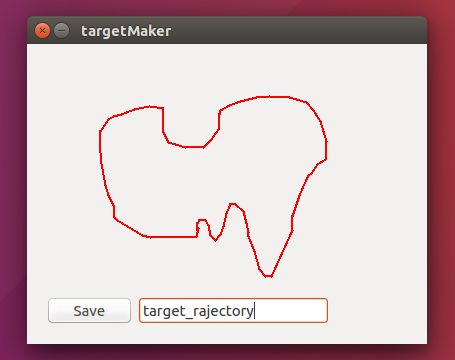
\includegraphics[scale=0.6]{../figures/targettrajectory.png}
 \caption{Éditeur de trajectoire}
 \label{fig:targettrajectory}
\end{figure}
Une interface graphique a été implémentée en Qt afin de créer des trajectoires à la souris. (Figure \ref{fig:targettrajectory})


\subsection{Expérimentation}
Observons ensuite le résultat de l'apprentissage des réseaux de neurones sur les données issues de la commande aléatoire.

\newcommand{\actu}[1]{#1_{\text{actuelle}}}
\newcommand{\target}[1]{#1_{\text{target}}}
\newcommand{\xactu}{\actu{X}}
\newcommand{\yactu}{\actu{Y}}
\newcommand{\vactu}{\actu{V}}
\newcommand{\vtarget}{\target{V}}
\newcommand{\oactu}{\actu{O}}
\newcommand{\otarget}{\target{O}}
\newcommand{\mpwekawidth}{.48\linewidth}
\newcommand{\incweka}[1]{\includegraphics[scale=0.5]{#1}}
\newcommand{\wecaption}[1]{\caption{#1.\footnotesize (Généré par Weka 3.8.1)\normalsize}}
\subsubsection{Test du réseau de neurones}
Afin de vérifier si le réseau de neurones implémenté ne contient pas d'erreur, il sera d'abord utilisé pour une Sphero virtuelle.
Un modèle très simple de Sphéro a été implémenté. Ce modèle ne simule pas la vitesse et l'inertie angulaire.
Le modèle est le suivant: Soit
\begin{itemize}
 \item $(\xactu, \yactu)$ la position actuelle en cm,
 \item $\vactu$ la vitesse actuelle en cm/s
 \item $\vtarget$ la vitesse commandée d'unité inconnue,
 \item $\oactu$ l'orientation en degrés,
 \item $\otarget$ l'orientation commandée en degrés,
 \item $T$ la période de streaming.
\end{itemize}
\[ \text{acceleration} = a(\vtarget - \vactu)\]
Où $a \in \mathbb{R}^{+}$ est un paramètre.
\[ \text{Nouvelle vitesse} = \vactu + \text{acceleration} \times T \]
Posons $d$ la différence entre $\otarget$ et $\oactu$, négatif si le sens de $\oactu \rightarrow \otarget$ est horlogique.
Alors
\[ \text{Nouvelle orientation} = \oactu + d \]
Nouvelle vitesse et Nouvelle orientation sont limitées selon un paramètre.
\begin{center}
 \begin{tabular}{ll}
  Nouvelle position = & $(\xactu + (\text{Nouvelle vitesse})\cos(\text{Nouvelle orientation})$,\\
   & $\yactu + \text{Nouvelle vitesse}\sin(\text{Nouvelle orientation}))$
 \end{tabular}
\end{center}

Deux réseaux de neurones ont été testés: le \rbf implémenté et le \mlp de Weka.
Le fonction d'activation des neurones cachés de Weka est la sigmoïde.
\[ f(x) = \frac{1}{1+e^{-x}} \]
Tandis que la fonction d'activation des neurones de sortie est une fonction linéaire.

\begin{figure}
 \begin{minipage}[c]{\mpwekawidth}
  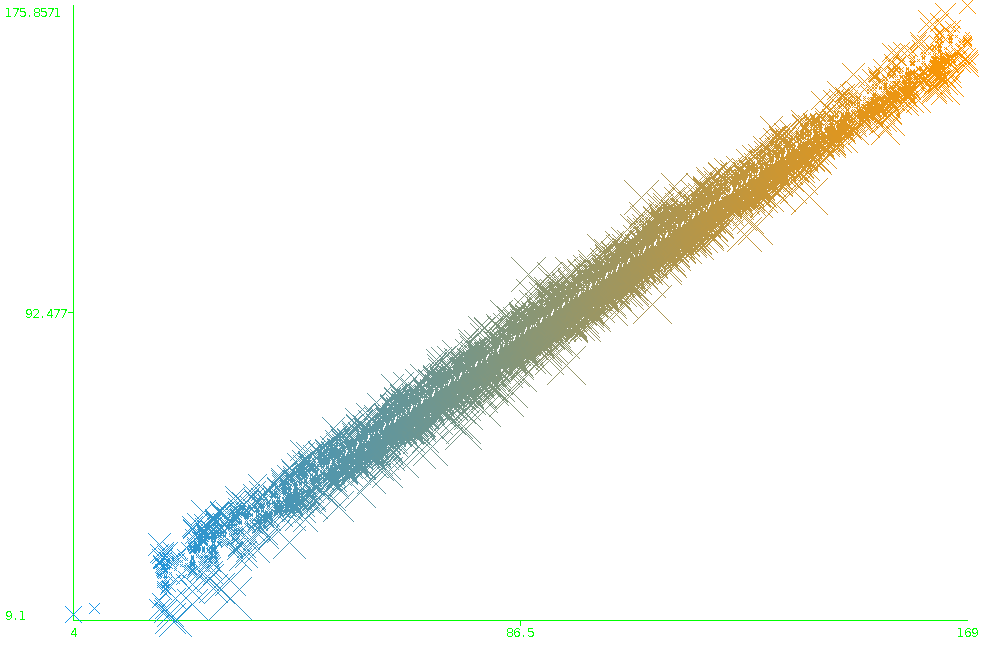
\includegraphics[width=\textwidth]{../figures/virtualResultSpeed.png}
 \end{minipage}
 \begin{minipage}[c]{\mpwekawidth}
  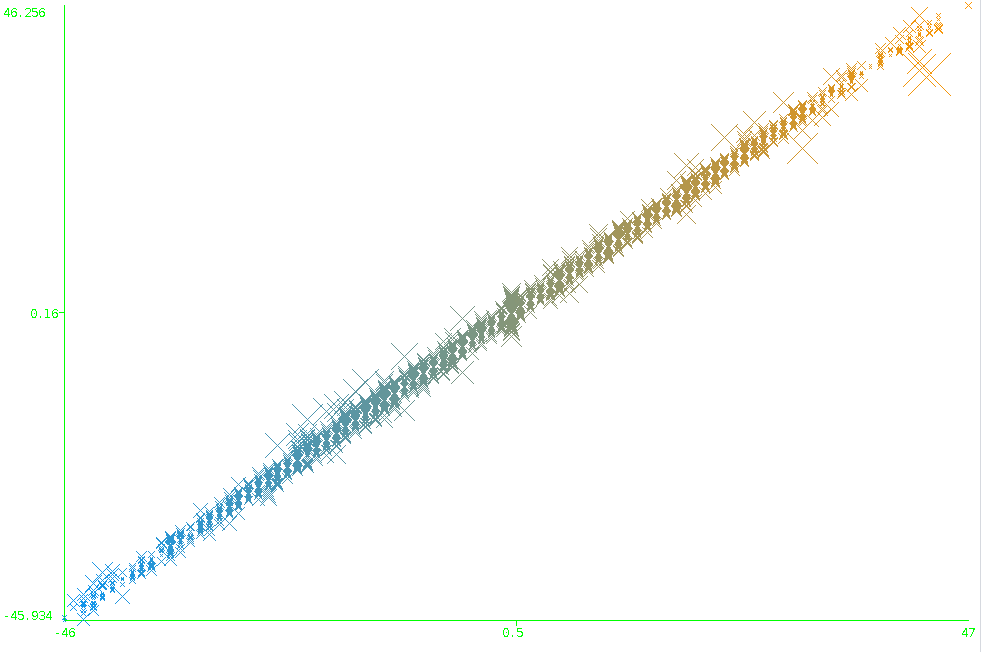
\includegraphics[width=\textwidth]{../figures/virtualHeadResult.png}
 \end{minipage}
 \wecaption{Nuages de point prédit/espéré sur la vitesse et l'orientation sur les données de la Sphero virtuelle}
 \label{we:virtualResult}
\end{figure}
Tous les deux étaient capables d'approximer ce modèle.
Pour que les résultats observés ne soient pas biaisées par le surajustement, la technique de 10fold cross-validation a été utilisée.
C'est à dire que la base de données est séparée en 10 ensembles de tailles égales.
Pour chaque ensemble, on construit le modèle sur les 90 autres pourcents de données et on utilise ces 10\% comme ensemble de test.
À la fin, on obtient un nuage de points (sortie espérée, sortie aproximée par le modèle) où nous pouvons, par exemple,
calculer le coefficient de corrélation pour avoir un indice sur la qualité du réseau de neurones pour ces données.
Comme sur la Figure \ref{we:virtualResult} où la corrélation est de 0,99 pour la vitesse et l'orientation.
Deux modèles différents ont été construit car il a été observé que le RBF implémenté est plus éfficace si il n'y a qu'une sortie à générer au lieu de deux.

\subsubsection{Observation des données réelles}
\begin{figure}
 \centering
 \incweka{../figures/targetxyvirtual.png}
 \wecaption{Nuage des positions à atteindre}
 \label{we:targetvirtual}
\end{figure}

Observons les données fournies par la commande aléatoire sur la véritable Sphero.
Dans la figure ? chaque point représentent la position que doit atteindre la Sphero $\frac{1}{f}$ secondes plus tard.
Pour chaque point, la Sphero est en (0,0) et est dirigée vers la droite, parallèle à l'axe x.
La couleur du point représente la valeur de l'orientation à commander.
Plus le ton est orangé, plus la valeur est grande.
On pourrait s'attendre à ce que plus le point est vers le haut, plus la valeur de head est grande, comme on peut l'observer sur les données de commande aléatoire sur la Sphero virtuelle. (Figure \ref{we:targetvirtual})
Mais ce n'est pas le cas, on observe un nuage de points aléatoires.
Pour chaque attribut qu'on peut prendre 2 à 2, on n'observe pas de pattern. TODO%TODO
Il nous faudrait pouvoir voir plus que 3 dimensions pour, peut-être, observer un pattern.
Mais en tout cas, il y en a un.
C'est ce que nous allons voir dans l'expérimentation sur les données réelles.

\subsubsection{Expérimentation sur données réelles}
Puisque cette expérience s'est déroulée en même temps que la phase de conception et de test du générateur de commande aléatoire,
il a fallut préparer un espace accessible sur une assez longue période.
La vitesse a été bridée et aucune caméra n'a été utilisée.
Dans ces conditions, une fréquence de 40Hz était trop élevée pour capturer les différences de positions car l'odométrie est capturée en nombre entier en cm.
Une fréquence de 5Hz était assez basse pour observer les différences de position mais assez élevée pour effectuer des mouvements fluides.
Pour toutes les obsevations effectuées, le RBF implémenté retournait toujours la moyenne des outputs.

\ssstitle{Avec données relatives à la position et l'orientation}
\begin{minipage}[c]{\mpwekawidth}
 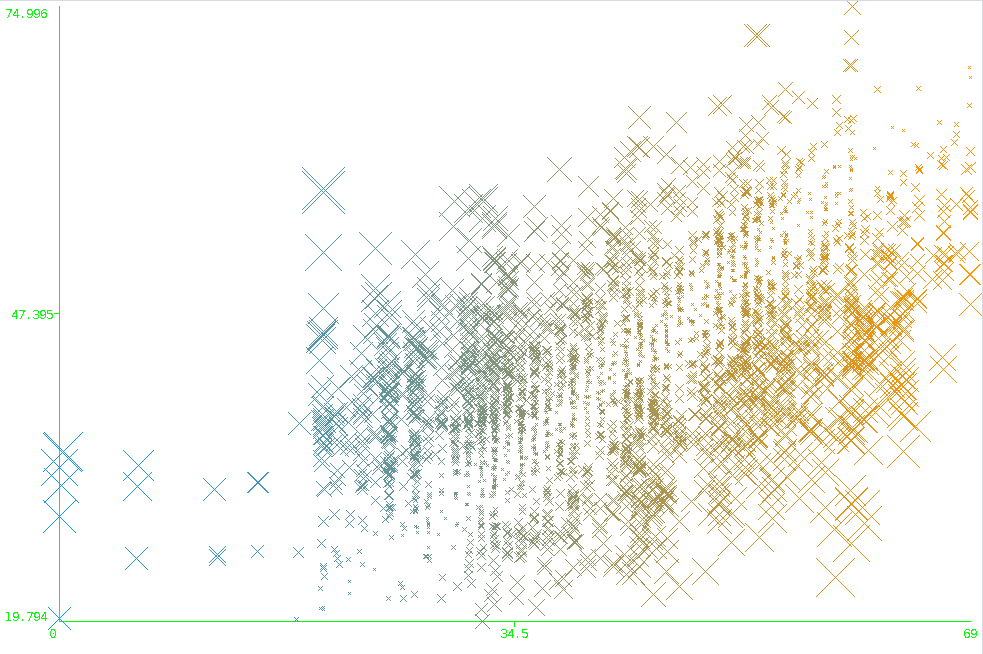
\includegraphics[width=\h]{../figures/speed121314N1500H20.png}
\end{minipage}
\begin{minipage}[c]{\mpwekawidth}
 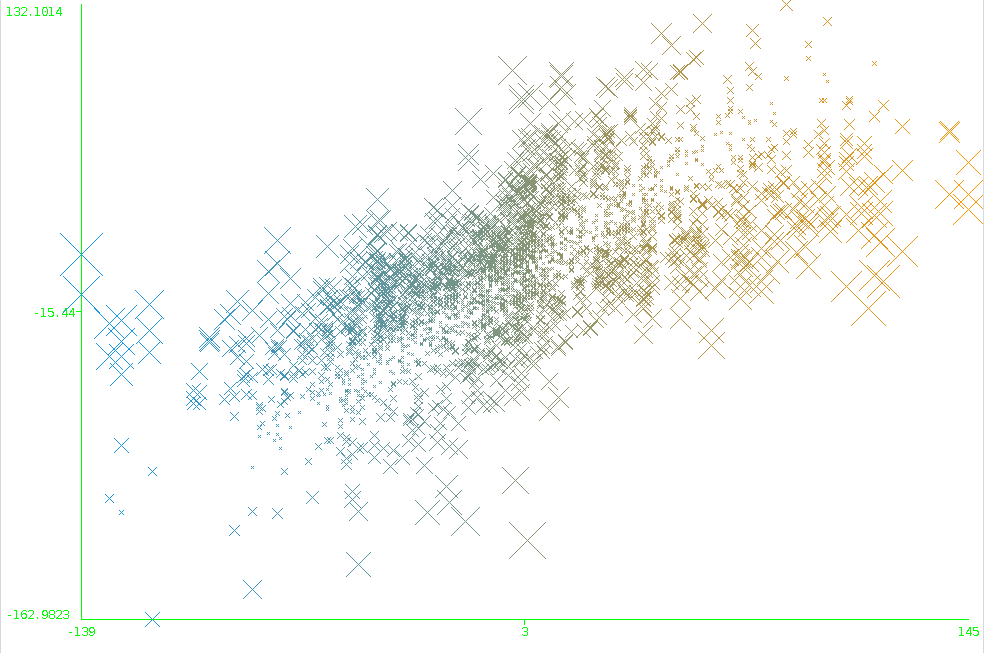
\includegraphics[width=\textwidth]{../figures/121314N1500H20.png}
\end{minipage}
\\
Ici, les données d'entrées sont relatifs à la position de la Sphero et à son orientation et sont normalisées.
Le réseau de neurones configuré sur Weka a une couche de 20 neurones cachés avec un learning rate (pas de gradient) de 0,3 et un nombre d'époques de 1500.
(C'est à dire que les données d'entrainement sont présentés 1500 fois aux réseaux de neurones).
Le coefficient de corrélation est de 0.5404 pour la vitesse et de 0,69 pour l'orientation.

\ssstitle{Ajout de la vitesse commandée en attribut}
\begin{minipage}[c]{\mpwekawidth}
 TODO %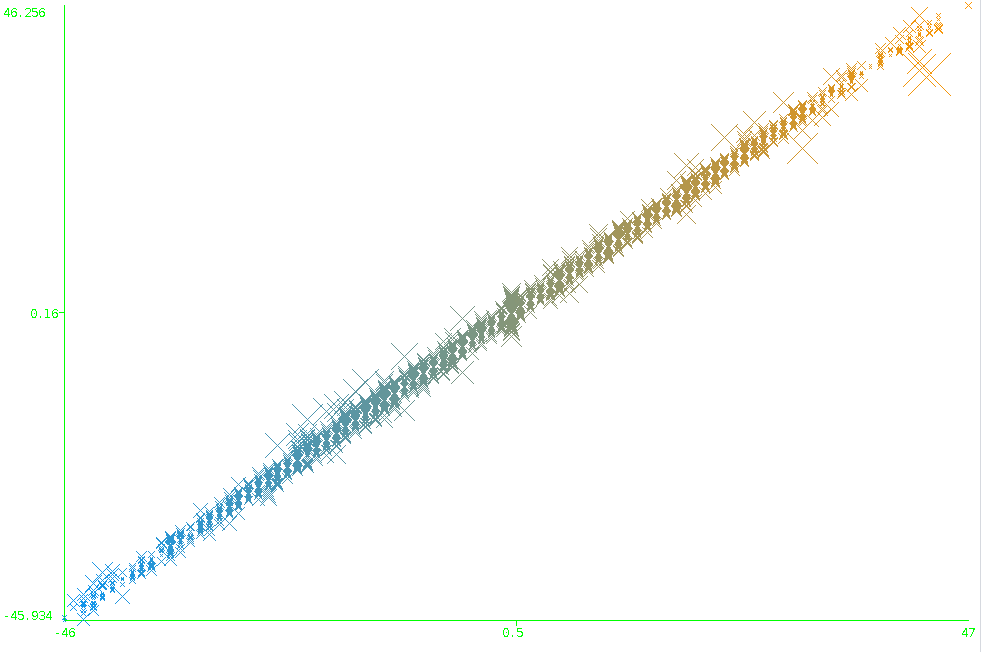
\includegraphics[width=\h]{../figures/virtualHeadResult.png}
\end{minipage}
\begin{minipage}[c]{\mpwekawidth}
 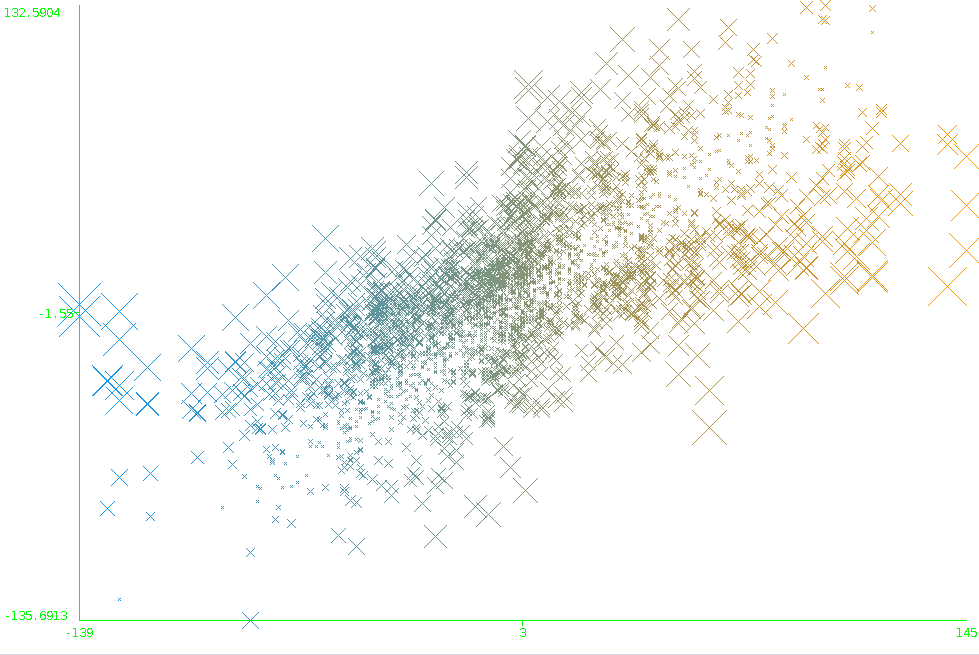
\includegraphics[width=\textwidth]{../figures/121314SpeedN1500H20.png}
\end{minipage}
\\
C'est ce que nous obtenons si on ajoute la vitesse commandée en attribut.
La configuration du réseau de neurones est la même que la précédente.
Le coefficient de corrélation est de ? pour la vitesse et de 0,72 pour l'orientation.

\ssstitle{Avec données relatives à la position et l'orientation et en mirroir sur l'axe x}
\ssstitle{Avec données relatives à la position et l'orientation, ordered speed en attribut et output non normalisé}
\ssstitle{Avec données relatives à la position et l'orientation, ordered speed en attribut et input non normalisé}
\ssstitle{Avec données relatives à la position et l'orientation, ordered speed en attribut, input et output non normalisés}


\section{Conclusion}
Malgré que le projet ne soit pas arrivé à son terme, nous avons découvert que pour pouvoir piloter une Sphero avec un réseau de neurone, nous avons besoin de nouveaux attributs ou d'une autre achitecture de réseau de neurones.
En effet, malgré tous les problèmes rencontrés nuisant à la qualité des données récoltées (section \ref{sec:choixdesign} et \ref{sec:choixdesign}) ,
un réseau de neurone devrait être capable d'approximer une fonction même avec des imprécisions, ou, du moins, de converger vers une autres solution que la moyenne de toutes les sorties.
Les autres attributs qui peuvent être ajoutées sont la vitesse à atteindre, l'inclinaison gauche-droite, l'inclinaison arrière-avant et les commandes précédentes.

\subsection*{Remerciements}
\noindent Je remercie Monsieur Pierre \textsc{Hauweele} de m'avoir proposé un projet qui est exactement dans le domaine que je voulais, de son aide et de la direction de mon projet.\\

\noindent Je remercie Monsieur Hadrien Mélot pour la direction de mon projet et de l'aide qu'il m'a apporté.\\

\noindent Je remercie Monsieur Tom Mens pour son feed-back et ses conseils sur la rédaction de ce rapport.\\

\noindent Je remercie Monsieur Gauvain Devillez pour m'avoir débloqué plusieurs fois dans la compilation et ses conseils.sec:realdataex

\bibliographystyle{unsrt-fr}%unsrt-fr pour reference fr par num. plainnat-fr ou frplain Pour reference fr par auteur et annee
\bibliography{../bibli}
\appendix

\section{Équations de rétropropagation d'un MLP}\label{sec:eqmlp}
La modification à apporter au poids $j$ du neurone $i$ vaut
\begin{equation}\label{eq:Delta}
 \Delta W_{ij} = -\eta\partiel{Q}{W_{ij}}
\end{equation}
\begin{equation}\label{eq:gradient}
 \partiel{Q}{W_{ij}} = \partiel{Q}{\phi_i} \partiel{\phi_i}{v_i} \partiel{v_i}{W_{ij}}
\end{equation}
Et on a posé
\begin{equation}\label{eq:deltai}
 \delta_i = \partiel{Q}{\phi_i} \partiel{\phi_i}{v_i}
\end{equation}
En reprenant \eqref{eq:gradient}, nous avons maintenant que
\begin{equation}\label{eq:graddelta}
 \partiel{Q}{W_{ij}} = \delta_i \partiel{v_i}{W_{ij}}
\end{equation}
Nous allons déterminer la valeur de $\delta_i$ et de $\partiel{v_i}{W_{ij}}$.
Commençons par déterminer $\partiel{v_i}{W_{ij}}$.
Soit $x_{ij}$ la $j$\textsuperscript{ième} entrée du neurone $i$,
\begin{equation}\label{eq:gradsum}
 \begin{split}
  \partiel{v_i}{W_{ij}} & = \partiel{(W_{i0}x_{i0})}{W_{ij}} + \partiel{(W_{i1}x_{i1})}{W_{ij}} + ... + \partiel{(W_{ij}x_{ij})}{W_{ij}} + ... + \partiel{(W_{im}x_{im})}{W_{ij}}\\
  ~ & = x_{ij}
  \end{split}
\end{equation}
Ensuite, déterminons la valeur de $\delta_i$ selon deux cas: si $i$ est un neurone de sortie et si $i$ est un neurone caché.\\

\textbf{Si le neurone $i$ est un neurone de sortie,}
\begin{equation}\label{eq:sortie1}
 \begin{split}
  \partiel{Q}{\phi_i} & = \frac{1}{2} \left( \partiel{(\phi_0 - s_0)^2}{\phi_i} + \partiel{(\phi_1 - s_1)^2}{\phi_i} + ... + \partiel{(\phi_i - s_i)^2}{\phi_i} + ... + \partiel{(\phi_l - s_l)^2}{\phi_i} \right)\\
  ~ & = \frac{1}{2}2(\phi_i - s_i)\partiel{(\phi_i - s_i)}{\phi_i}\\
  ~ & = (\phi_i - s_i)
 \end{split}
\end{equation}
Soit $\phi'$ la dérivée de $\phi$,
\begin{equation}\label{eq:sortie2}
 \partiel{\phi_i}{v_i} = \phi'(v_i)
\end{equation}
Par \eqref{eq:sortie1} et \eqref{eq:sortie2}, on a
\[\delta_i = (\phi_i - s_i)\phi'(v_i)\]\\

\textbf{Si le neurone $i$ est un neurone caché,}
alors soit $n$ le nombre de neurones de la couche suivante (plus proche des neurones de sorties), soit $k$ un neurone de la couche suivante, on sait que $Q$ est fonction composée,
dépendant de $\phi_k$, lui-même dépendant de $v_k$, dépendant lui-même de $\phi_i$.
C'est pour cela qu'en appliquant le théorème de dérivée des fonctions composées,
\begin{equation}\label{eq:cache1beforebefore}
 \partiel{Q}{\phi_i} = \sum_{k=1}^{n} \partiel{Q}{\phi_k} \partiel{\phi_k}{v_k} \partiel{v_k}{\phi_i}
\end{equation}
Si on subsitue \eqref{eq:deltai} dans \eqref{eq:cache1beforebefore},
\begin{equation}\label{eq:cache1before}
 \partiel{Q}{\phi_i} = \sum_{k=1}^{n} \delta_k \partiel{v_k}{\phi_i}
\end{equation}
Or $\phi_i$ est l'entrée du neurone $k$ recevant la sortie du neurone $i$. Posons $W_{ki}$ le poids que $k$ attribue à $\phi_i$.
On peut alors continuer à développer \eqref{eq:cache1before} comme suit:
\begin{equation}\label{eq:cache1}
 \partiel{v_k}{\phi_i} = \partiel{W_{ki}\phi_i}{\phi_i} = W_{ki}
\end{equation}
Pour la valeur de $\partiel{\phi_i}{v_i}$, nous pouvons reprendre \eqref{eq:sortie2}.
Et du coup, \[\delta_i = \phi_i'(v_i) \sum_{k=1}^{n} \delta_k W_{ki}\]

Nous connaissons maitenant la modification à appliquer sur $W_{ij}$. Pour résumé, subsituons $\delta_i$ et \eqref{eq:gradsum} à \eqref{eq:gradient},
\begin{equation}\label{eq:subgradient}
 \partiel{Q}{W_{ij}} = \delta_i x_{ij}
\end{equation}
Qu'on subsitue à \eqref{eq:Delta} et nous avons enfin
\begin{equation}\label{eq:mlpretro}
 \Delta W_{ij} = -\eta \delta_i x_{ij} \text{~où~}\left\{
  \begin{array}{lll}
   \delta_i & = (\phi_i - s_i)\phi'(v_i) & \text{Si~} i \text{~est un neurone de sortie}\\
   \delta_i & = \phi_i'(v_i) \sum_{k=1}^{n} \delta_k W_{ki} & \text{Si~} i \text{~est un neurone caché}
  \end{array}
 \right.
\end{equation}

\section{Équation de rétropropagation d'un RBF}\label{sec:eqrbf}
Les modifications à apporter aux paramètres d'un neurone $i$ vaut
\begin{equation}\label{eq:modifpoid}
 \Delta W_{ij} = -\eta \partiel{Q}{W_{ij}}
\end{equation}
\begin{equation}\label{eq:modifmu}
 \Delta \mu_{ij} = -\eta \partiel{Q}{\mu_{ij}}
\end{equation}
\begin{equation}\label{eq:modifsigma}
 \Delta \sigma_{ij} = \eta \partiel{Q}{\sigma_{ij}}
\end{equation}

D'abord déterminons le facteur $\partiel{Q}{W_{ij}}$ dans \eqref{eq:modifpoid}.
On est dans le cas où $i$ est un neurone de sortie.
Par \eqref{eq:Q}, $Q$ dépend de $\phi_i$.
Par \eqref{eq:sortiephi}, $phi_i$ dépend de $W_{ij}$.
Par le théorème de dérivée des fonctions composés,
\begin{equation}\label{eq:rbfsortie}
 \partiel{Q}{W_{ij}} = \partiel{Q}{\phi_i} \partiel{\phi_i}{W_{ij}}
\end{equation}
Par \eqref{eq:sortie1}, on sait que
\[\partiel{Q}{\phi_i} = (\phi_i - s_i)\]
Ensuite,
\begin{equation}\label{eq:poidgrad}
 \begin{split}
  \partiel{\phi_i}{W_{ij}} & = \partiel{\frac{\sum_{r=1}^{m}W_{ir}x_{j}}{\factnorm}}{W_{ij}} \text{\hspace{1cm} par \eqref{eq:sortiephi}}\\
  ~ & = \frac{1}{\factnorm} \partiel{\sum_{r=1}^{m}W_{ir}x_{j}}{W_{ij}}\\
  ~ & = \frac{x_j}{\factnorm}
 \end{split}
\end{equation}
Subsituons \eqref{eq:sortie1} et \eqref{eq:poidgrad} dans \eqref{eq:rbfsortie}.
\begin{equation}\label{eq:sortiegrad}
 \partiel{Q}{W_{ij}} = (\phi_i - s_i) \frac{x_j}{\factnorm}
\end{equation}
Et \eqref{eq:sortiegrad} dans \eqref{eq:modifpoid},
\[\Delta W_{ij} = -\eta (\phi_i - s_i) \frac{x_j}{\factnorm}\]\\

Déterminons maintenant le facteur $\partiel{Q}{\mu_{ik}}$ dans \eqref{eq:modifmu}. On est dans le cas où $i$ est un neurone caché.
$Q$ dépend de $\phi_i$ qui lui-même est fonction de $\mu_{ik}$ \eqref{eq:cachephi}. Par le théorème de dérivée de fonction composés,
\begin{equation}\label{eq:composemu}
 \partiel{Q}{\mu_{ik}} = \partiel{Q}{\phi_i} \partiel{\phi_i}{\mu_{ik}}
\end{equation}
On va déterminer la valeur de $\partiel{Q}{\phi_i}$ et puis de $\partiel{\phi_i}{\mu_{ik}}$.
Soit $j$ un neurone de sortie. On sait que $Q$ dépend de tous les $\phi_j$ et les $\phi_j$ dépendent de $\phi_i$. On sait donc que
\begin{equation}\label{eq:mufact1}
 \partiel{Q}{\phi_i} = \sum_{j} \partiel{Q}{\phi_j}\partiel{\phi_j}{\phi_i}
\end{equation}
Par \eqref{eq:sortie1}, on sait que
\[\partiel{Q}{\phi_j} = (\phi_j - s_j)\]
Et posons $x_r$ l'entrée de $j$ provenant de $i$, c'est à dire $\phi_i = x_r$.
Posons $n$ la dimension de l'entrée de $j$.
Posons aussi $R = \sum_{k=1}^{n}x_k$.
Pour trouver la valeur de $\partiel{\phi_j}{\phi_i}$, nous aurons besoin de trouver $\partiel{\frac{1}{R}}{x_k}$.
\begin{equation}\label{eq:1sr}
 \begin{split}
 \partiel{\frac{1}{R}}{x_k} & = \frac{-1}{R^2}\partiel{R}{x_k}\\
 ~ & = \frac{-1}{R^2}
 \end{split}
\end{equation}
Dès lors, utilisons \eqref{eq:1sr} pour simplifier l'équation suivante;
\begin{equation}\label{eq:phiiphij}
 \begin{split}
 \partiel{\phi_j}{\phi_i} & = \partiel{\phi_j}{x_r}\\
 ~ & = \partiel{\left(\frac{\sum_{k=1}^{n}W_{jk}x_k}{\sum_{k=1}{n}x_k}\right)}{x_r}\\
 ~ & = \partiel{\left(\frac{W_{j1}x_1}{R}\right)}{x_r} + \partiel{\left(\frac{W_{j2}x_2}{R}\right)}{x_r} + ... + \partiel{\left(\frac{W_{jr}x_r}{R}\right)}{x_r} + .. + \partiel{\left(\frac{W_{jn}x_n}{R}\right)}{x_r}\\
 ~ & = (W_{j1}x_1)\frac{-1}{R^2} + (W_{j2}x_2)\frac{-1}{R^2} + ... + \left[(W_{jr}x_r)\partiel{\frac{1}{R}}{x_r}+\partiel{(W_{jr}x_r)}{x_r}\frac{1}{R}\right] + ... + (W_{jn}x_n)\frac{-1}{R^2}\\
 ~ & = \left(\sum_{k=1}^{n}W_{jk}x_k\frac{-1}{R^2}\right)-W_{jr}x_r\frac{-1}{R^2} + \left[(W_{jr}x_r)\frac{-1}{R^2}+W_{jr}\frac{1}{R}\right]\\
 ~ & = \frac{-1}{R^2} \left[\left(\sum_{k=1}^{n}W_{jk}x_k\right)-W_{jr}x_r + (W_{jr}x_r) + W_{jr}(-R)\right]\\
 ~ & = \frac{1}{R^2} \left(W_{jr}R - \sum_{k=1}^{n}W_{jk}x_k\right)
 \end{split}
\end{equation}
On substitue \eqref{eq:sortie1} et \eqref{eq:phiiphij} dans \eqref{eq:mufact1} pour obtenir
\begin{equation}\label{eq:mufacto1}
 \partiel{Q}{\phi_i} = \sum_{j} (\phi_j - s_j) \frac{1}{R^2} \left(W_{jr}R - \sum_{k=1}^{n}W_{jk}x_k\right)
\end{equation}

Si nous calculons $\partiel{\phi_i}{\mu_{ik}}$, nous obtenons
\begin{equation}\label{eq:mufacto2}
 \partiel{\phi_i}{\mu_{ik}} = \phi_i \frac{x_k-\mu_{ik}}{\sigma_{ik}^2}
\end{equation}
Et en substituant \eqref{eq:mufacto1} et \eqref{eq:mufacto2} dans \eqref{eq:composemu},
\[\partiel{Q}{\mu_{ik}} = \left[\sum_{i}(\phi_j - s_j) \frac{1}{R^2} \left(W_{jr}R - \sum_{k=1}^{n}W_{jk}x_k\right)\right] \phi_i\frac{x_k-\mu_{ik}}{\sigma_{ik}^2}\]
Qu'on substitue dans \eqref{eq:modifmu}, on obtient la modification à appliquer sur $\mu_{ik}$:
\[\Delta\mu_{ik} = -\eta \left[\sum_{i}(\phi_j - s_j) \frac{1}{R^2} \left(W_{jr}R - \sum_{k=1}^{n}W_{jk}x_k\right)\right] \phi_i\frac{x_k-\mu_{ik}}{\sigma_{ik}^2}\]

Enfin déterminons le facteur $\partiel{Q}{\sigma_{ik}}$ dans \eqref{eq:modifsigma}. On est dans le cas où $i$ est un neurone caché.
$Q$ dépend de $\phi_i$ qui lui-même est fonction de $\sigma_{ik}$. Par le théorème de dérivée de fonction composés,
\begin{equation}\label{eq:composesigma}
 \partiel{Q}{\sigma_{ik}} = \partiel{Q}{\phi_i} \partiel{\phi_i}{\sigma_{ik}}
\end{equation}
Si nous calculons $\partiel{\phi_i}{\sigma_{ik}}$, nous obtenons
\begin{equation}\label{eq:sigmafacto2}
 \partiel{\phi}{\sigma_{ik}} = \phi_i \frac{(x_k-\mu_{ik})^2}{\sigma_{ik}^3}
\end{equation}
On peut substituer \eqref{eq:mufacto1} et \eqref{eq:sigmafacto2} dans \eqref{eq:composesigma}:
\[\left[\sum_{i}(\phi_j - s_j) \frac{1}{R^2} \left(W_{jr}R - \sum_{k=1}^{n}W_{jk}x_k\right)\right] \phi_i \frac{(x_k-\mu_{ik})^2}{\sigma_{ik}^3}\]
Qu'on substitue dans \eqref{eq:modifsigma}, on obtient la modification à appliquer sur $\sigma_{ik}$:
\[\Delta \sigma_{ik} = -\eta \left[\sum_{i}(\phi_j - s_j) \frac{1}{R^2} \left(W_{jr}R - \sum_{k=1}^{n}W_{jk}x_k\right)\right] \phi_i \frac{(x_k-\mu_{ik})^2}{\sigma_{ik}^3}\]

\end{document}
